\chapter{Kuisioner Pengguna}


\begin{figure}[]
	\centering
	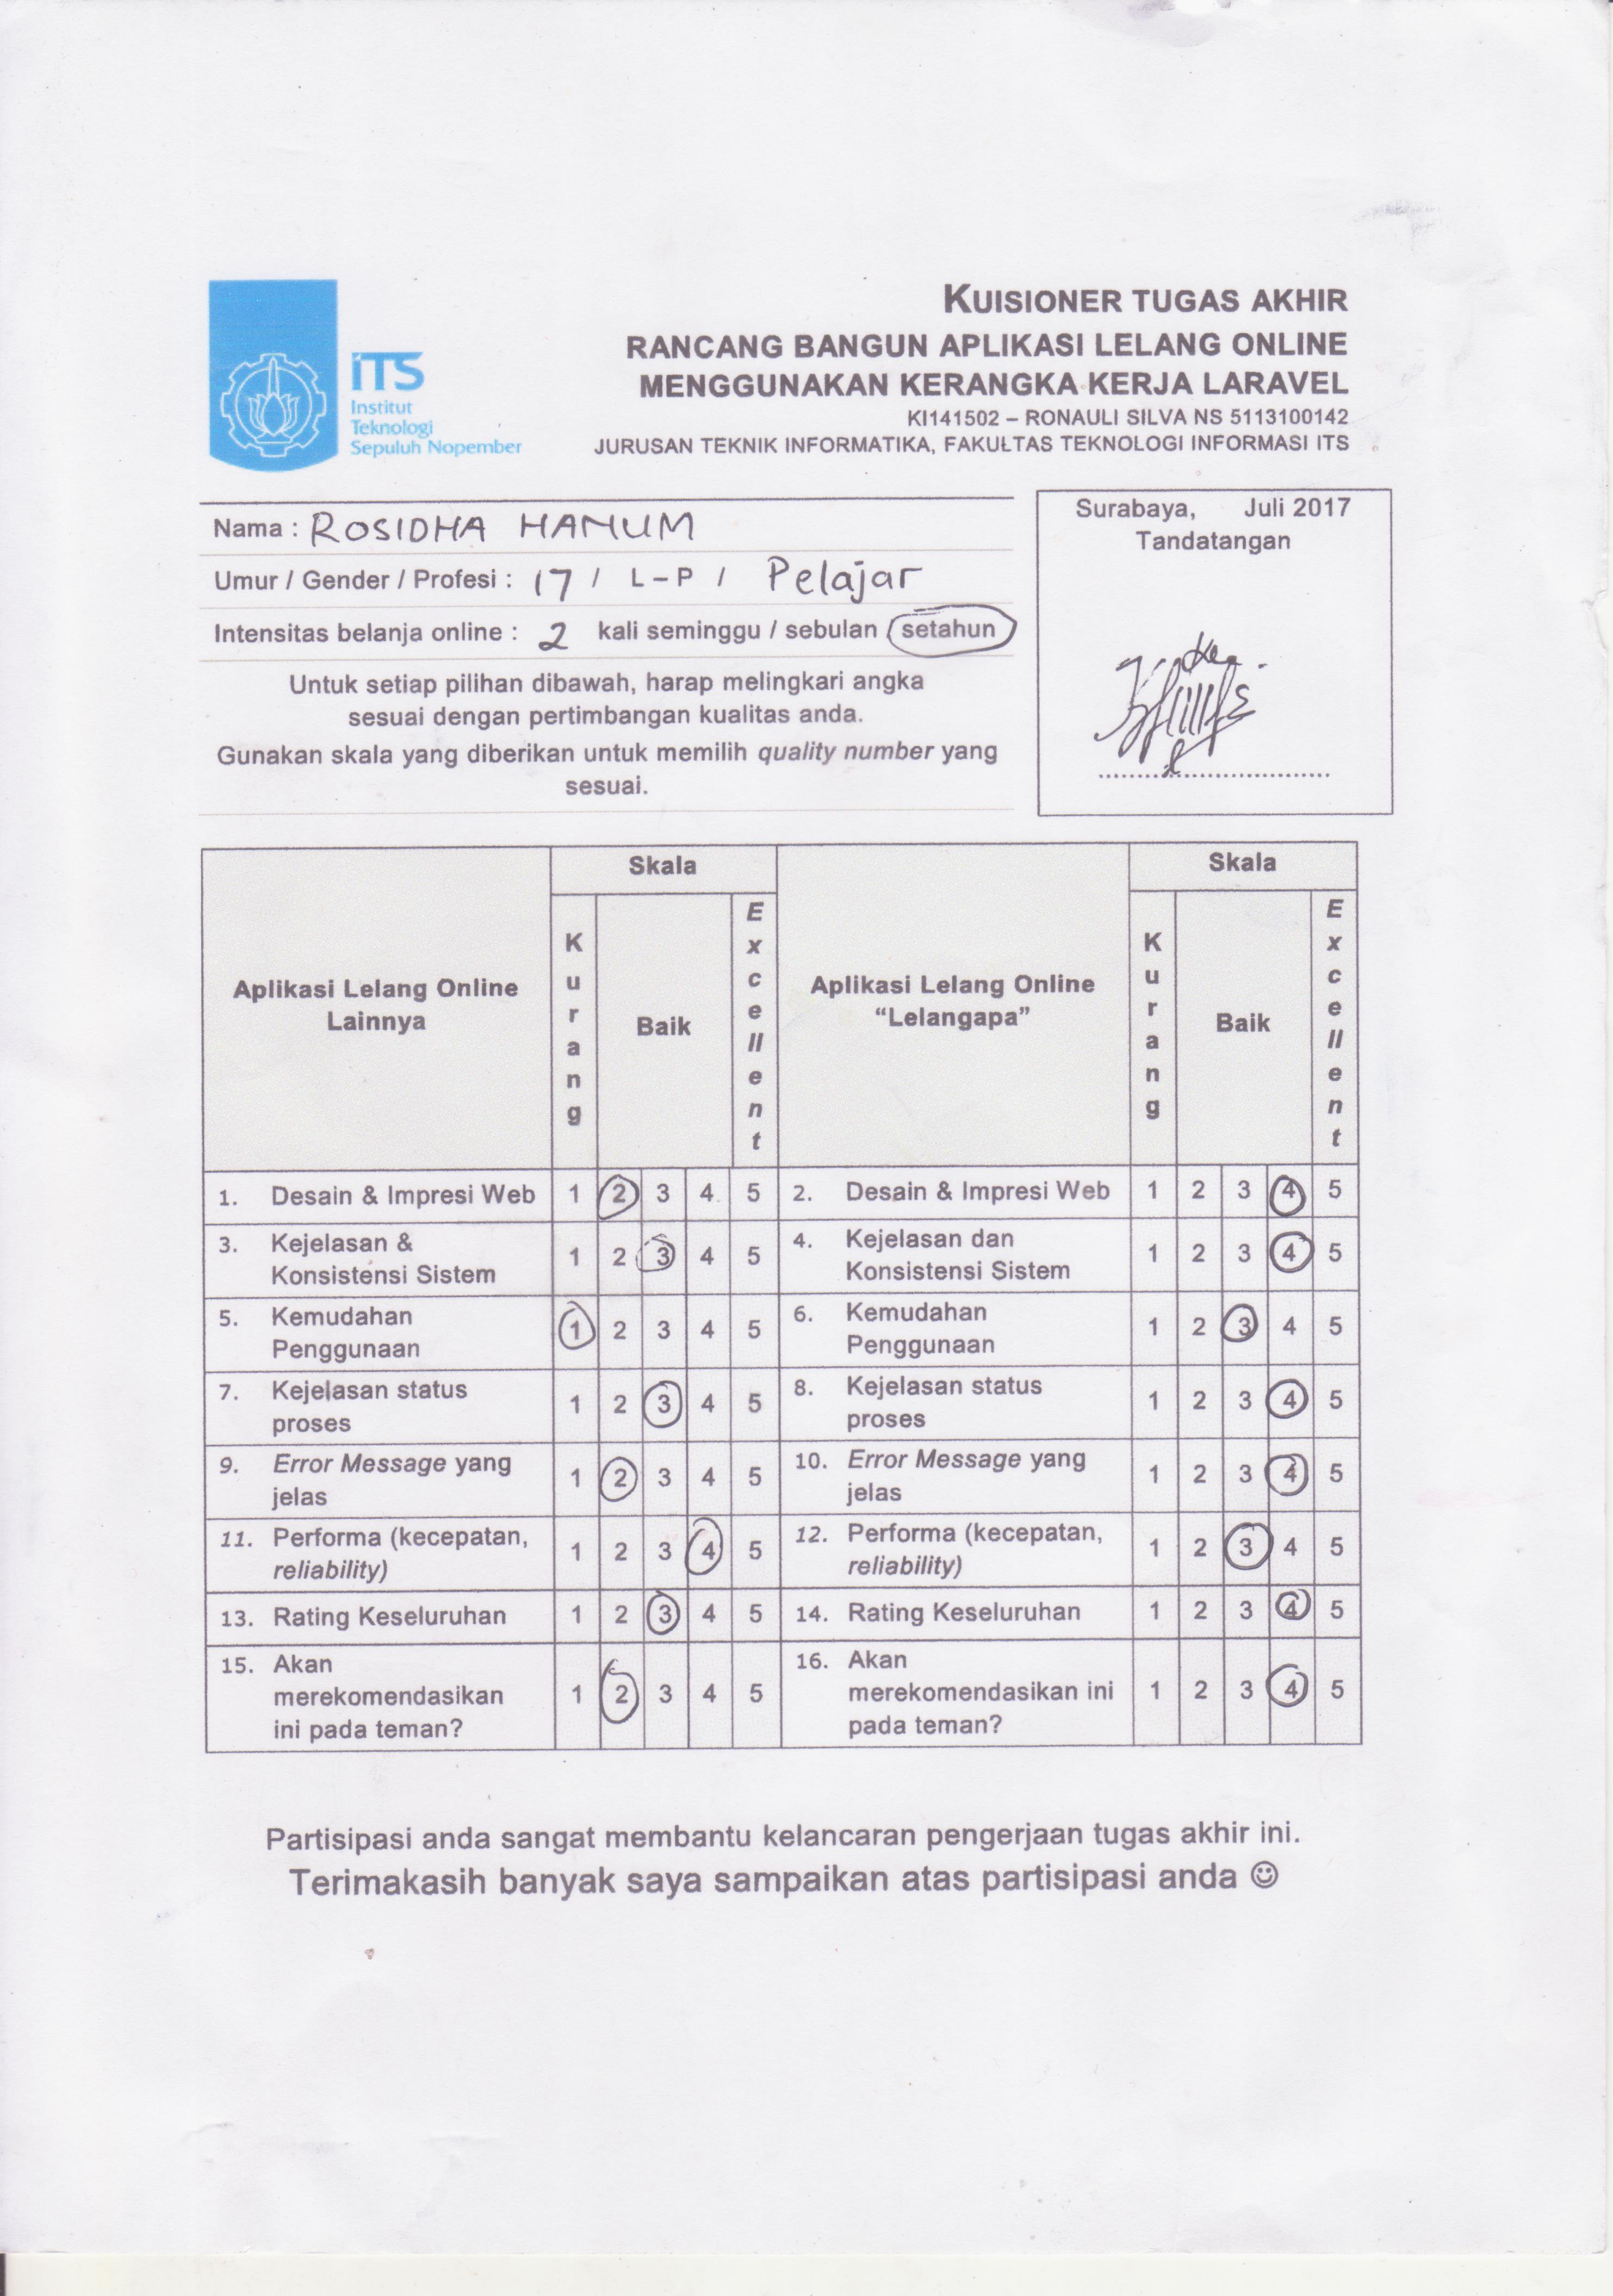
\includegraphics[width=\textwidth]{images/bab5/ujipengguna/1.jpg}
	\caption{Kuisioner Pengguna 1}
	\label{quest-1}
\end{figure}
\begin{figure}[]
	\centering
	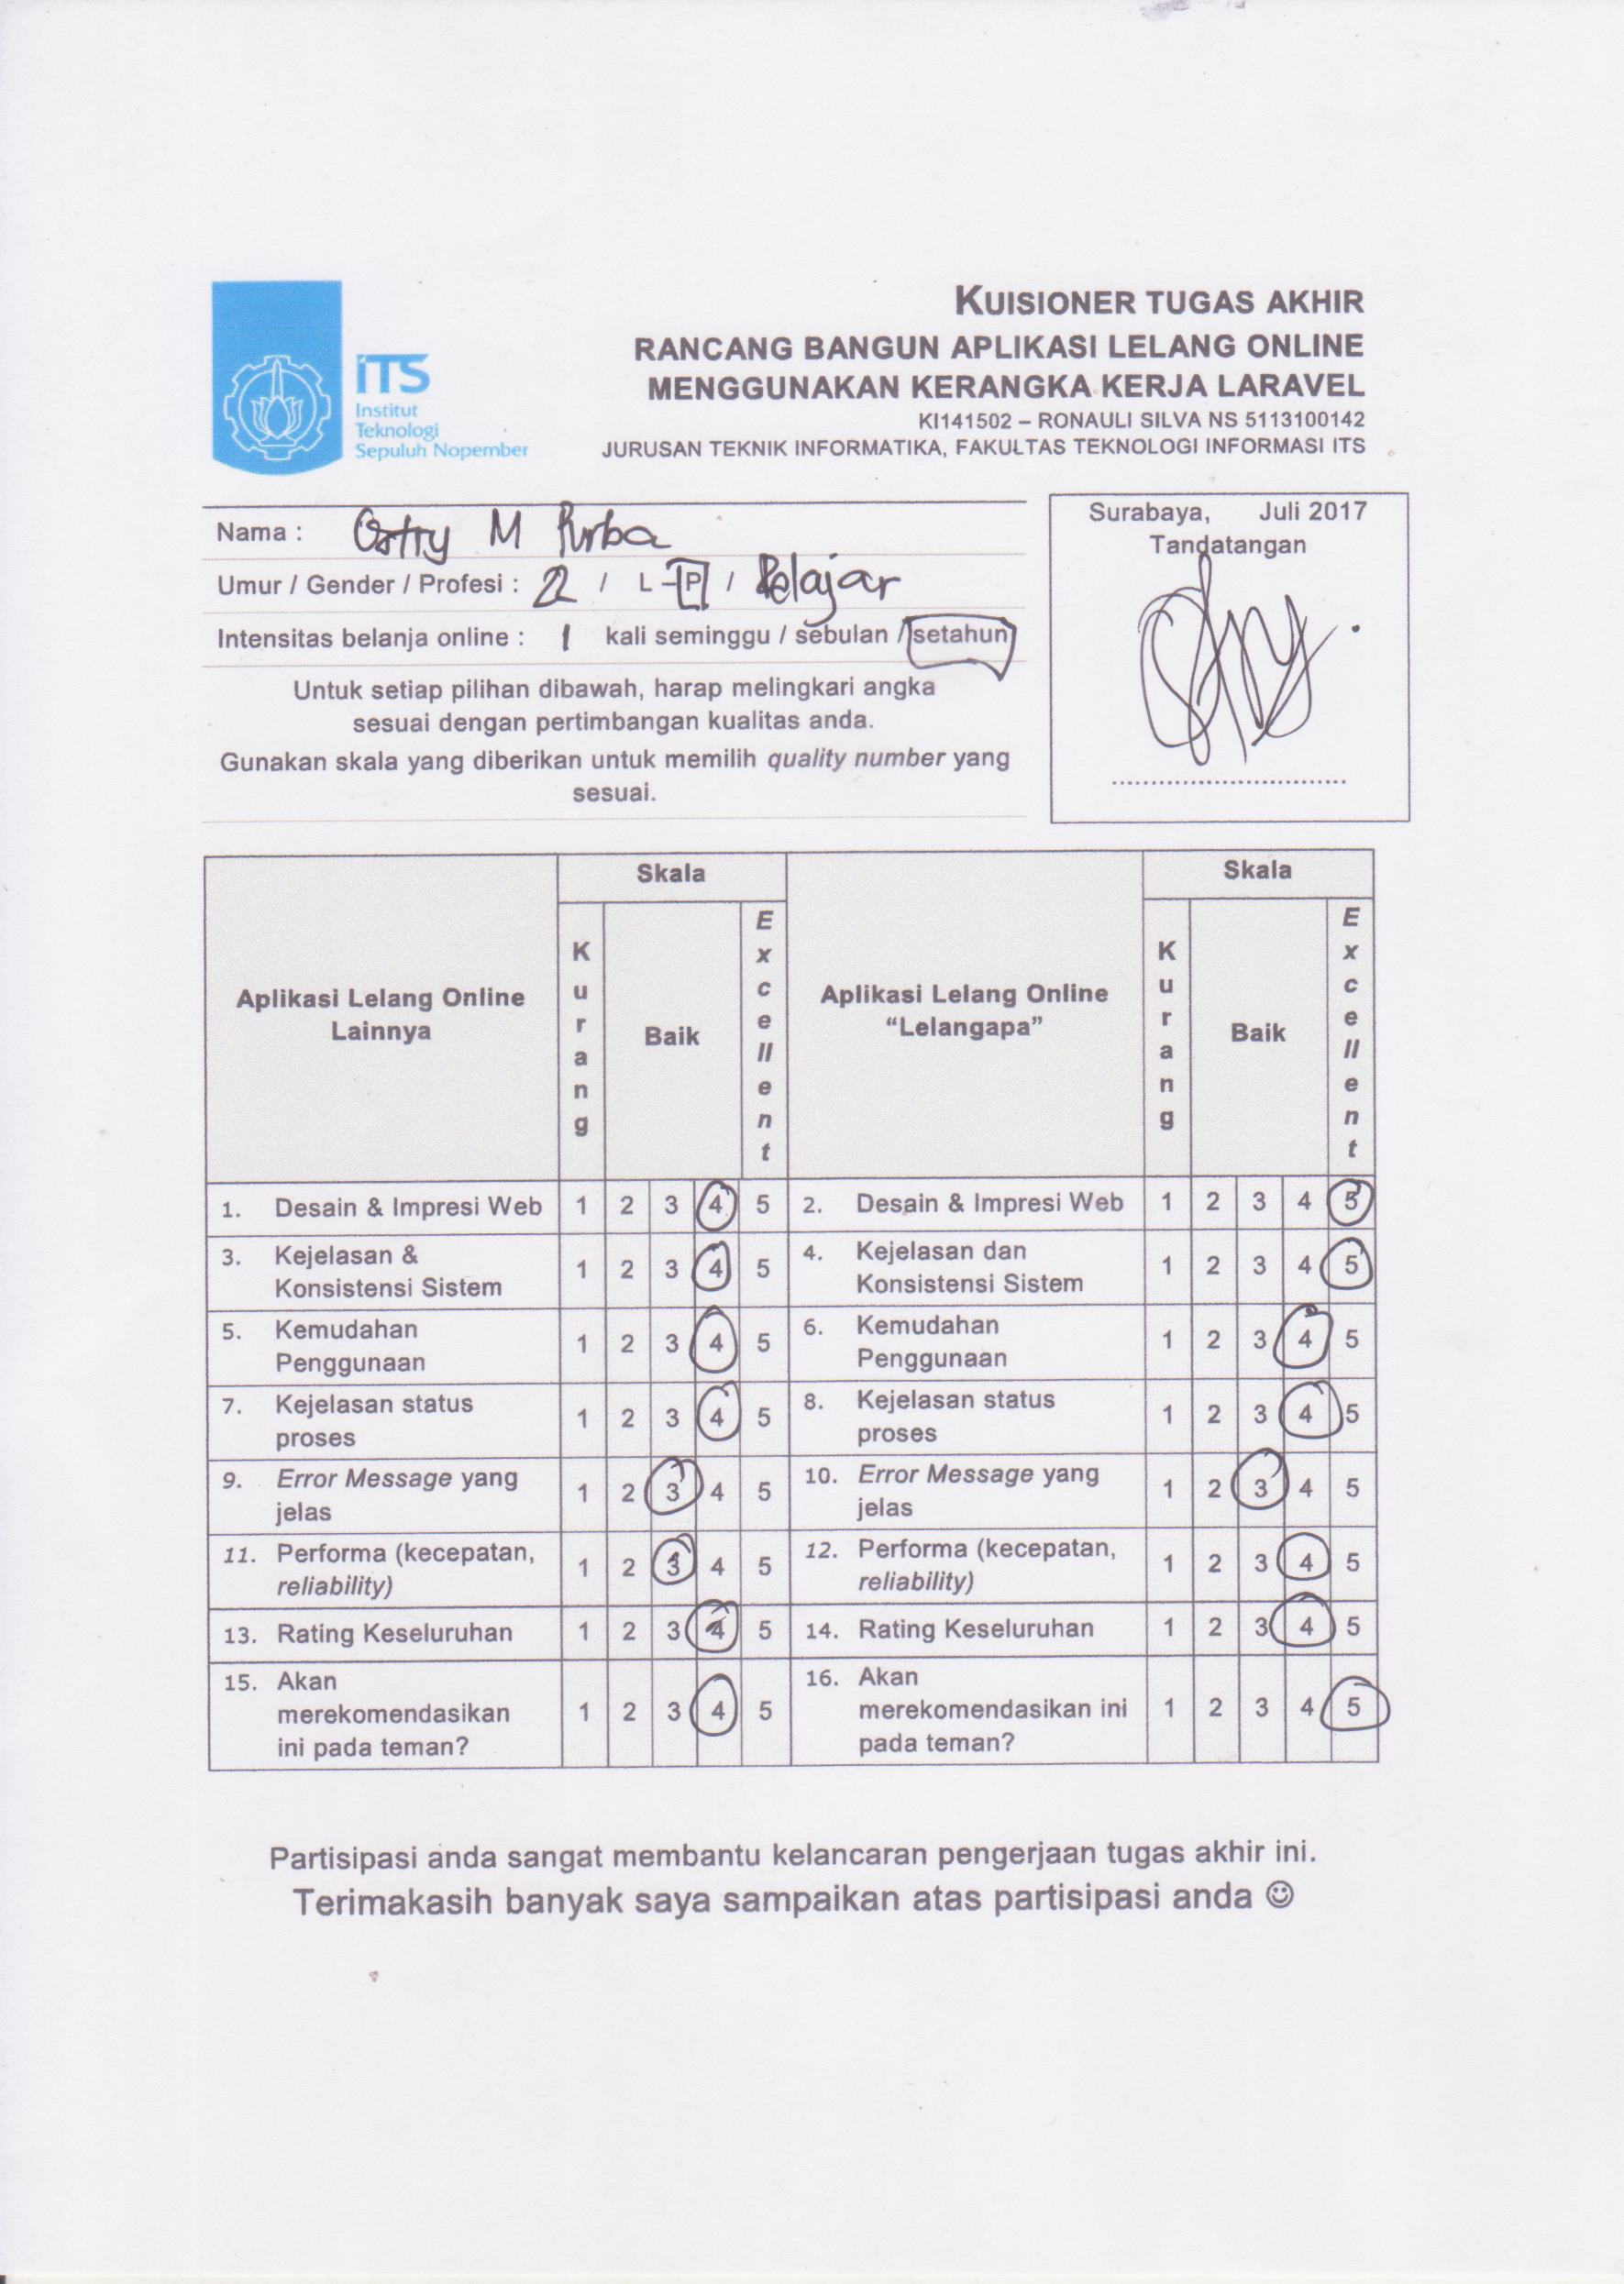
\includegraphics[width=\textwidth]{images/bab5/ujipengguna/2.jpg}
	\caption{Kuisioner Pengguna 2}
	\label{quest-2}
\end{figure}
\begin{figure}[]
	\centering
	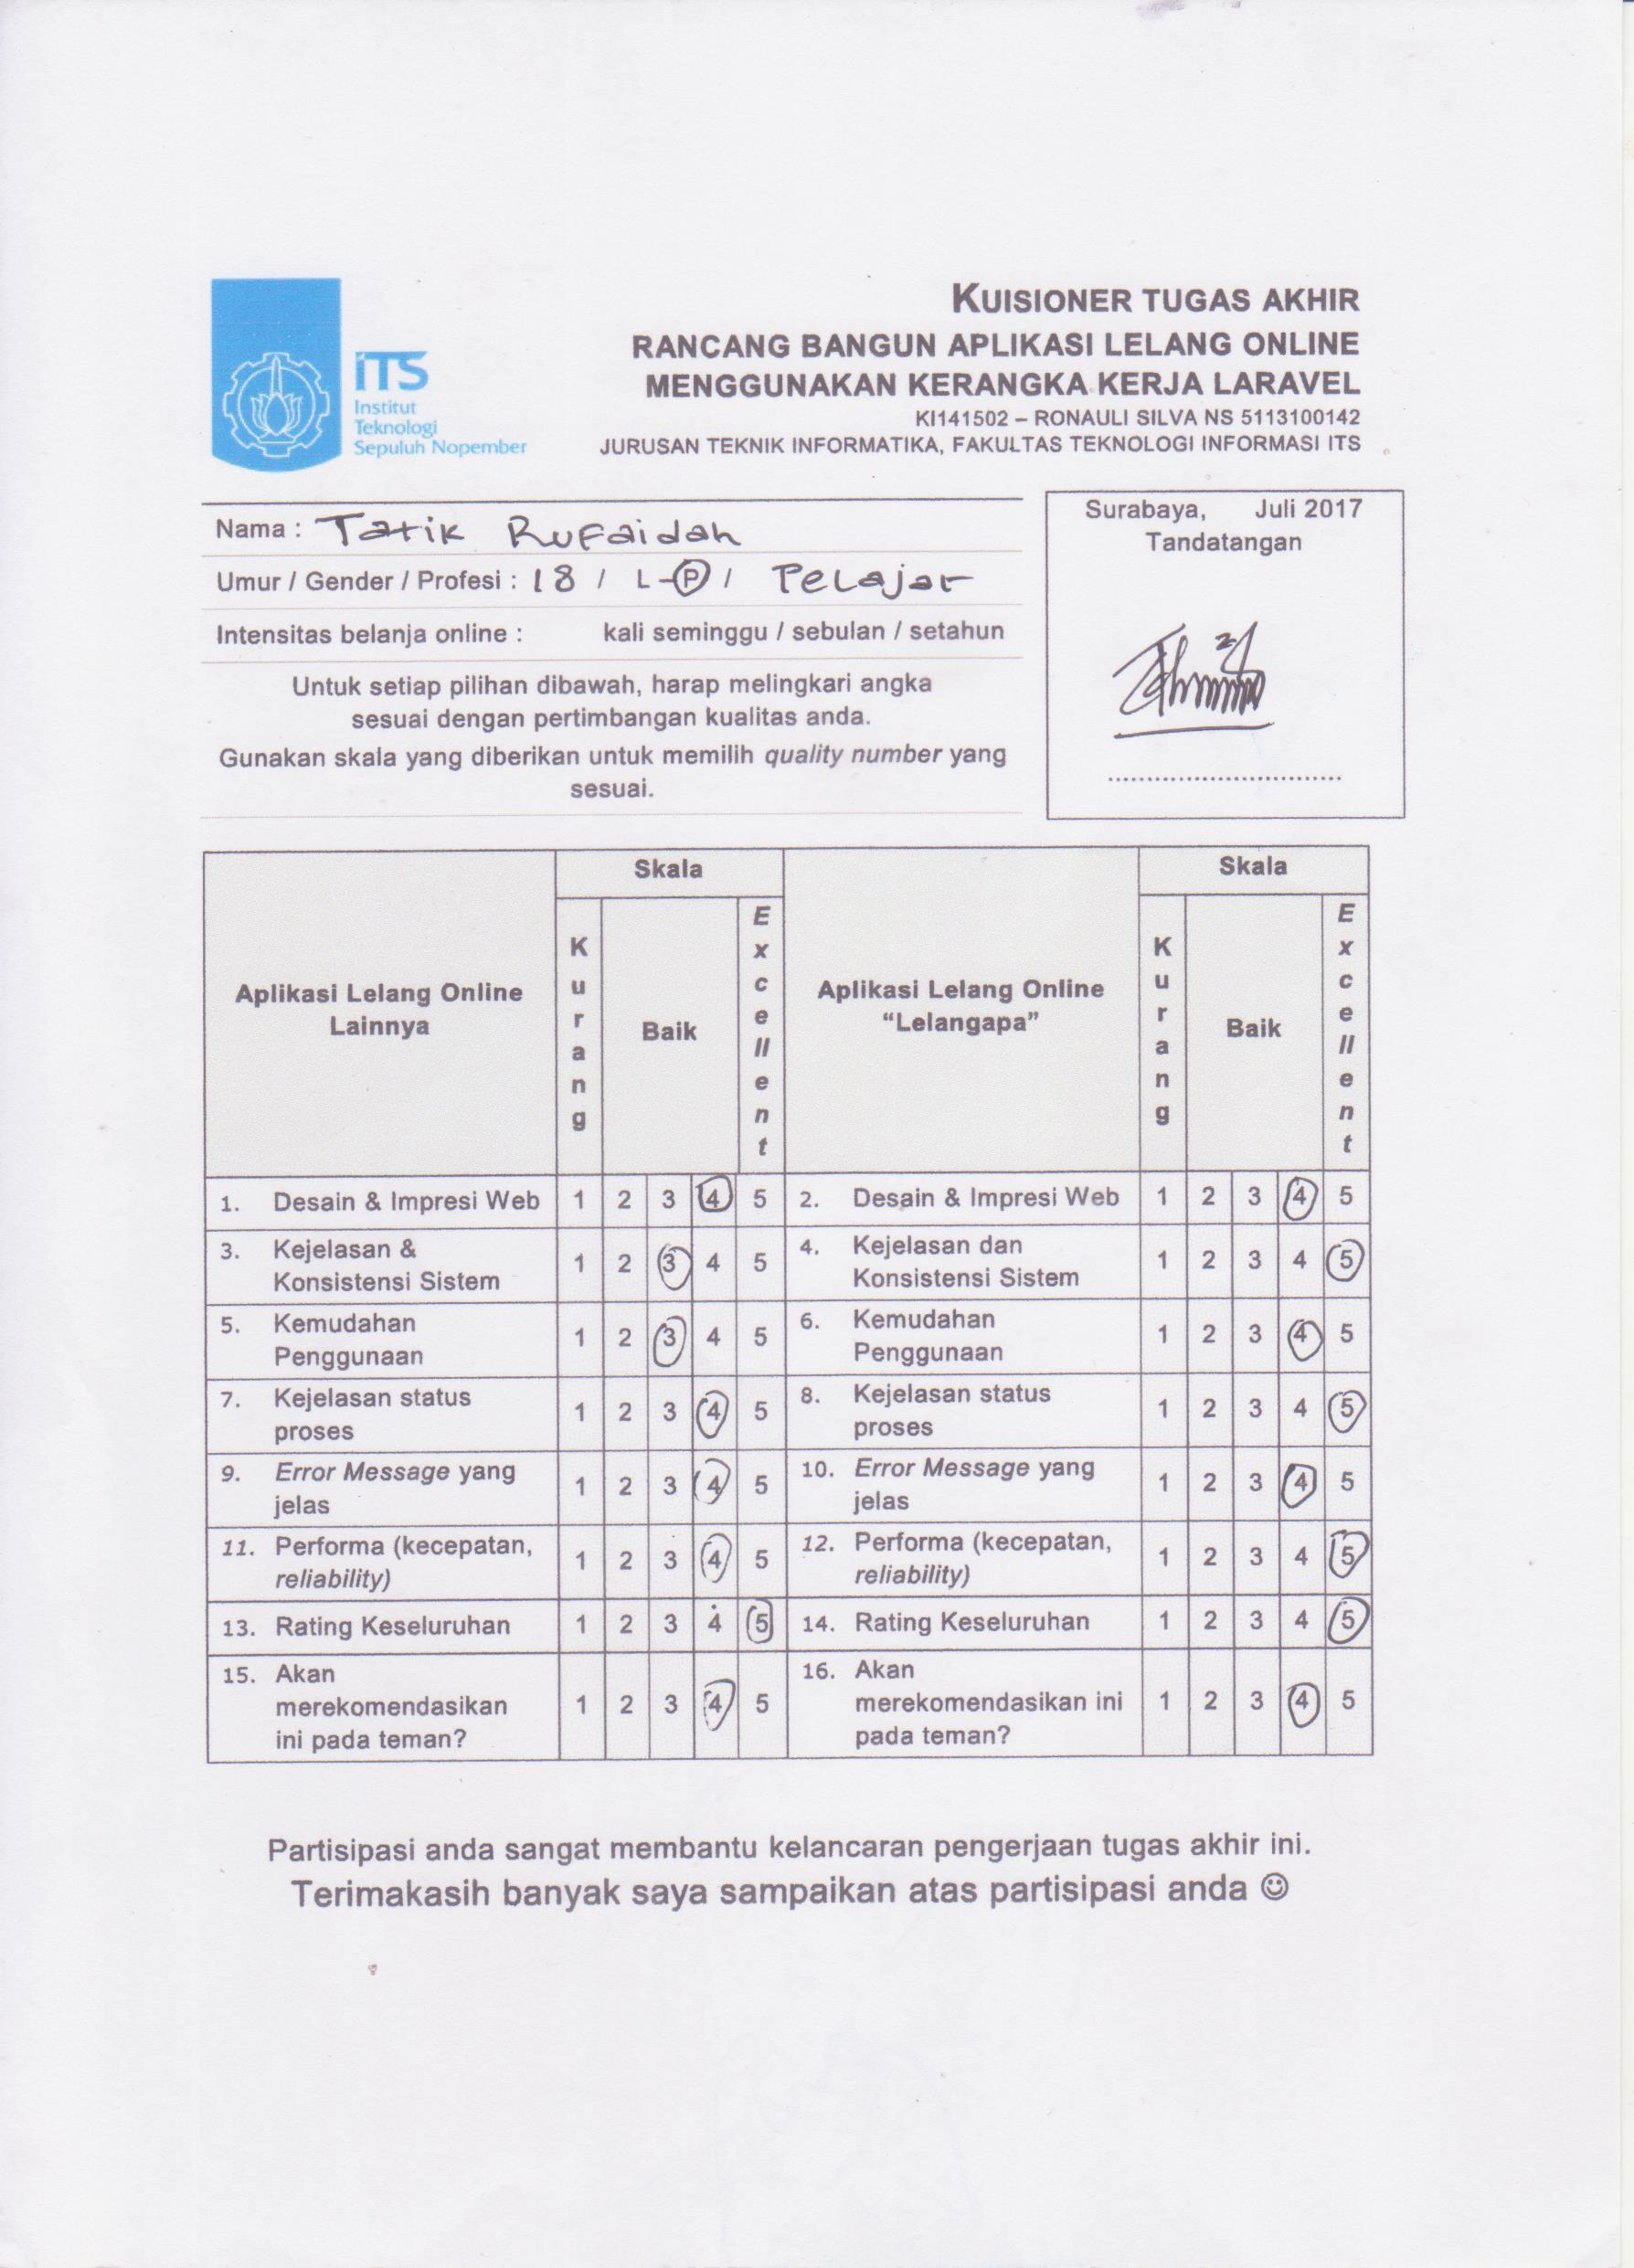
\includegraphics[width=\textwidth]{images/bab5/ujipengguna/3.jpg}
	\caption{Kuisioner Pengguna 3}
	\label{quest-3}
\end{figure}
\begin{figure}[]
	\centering
	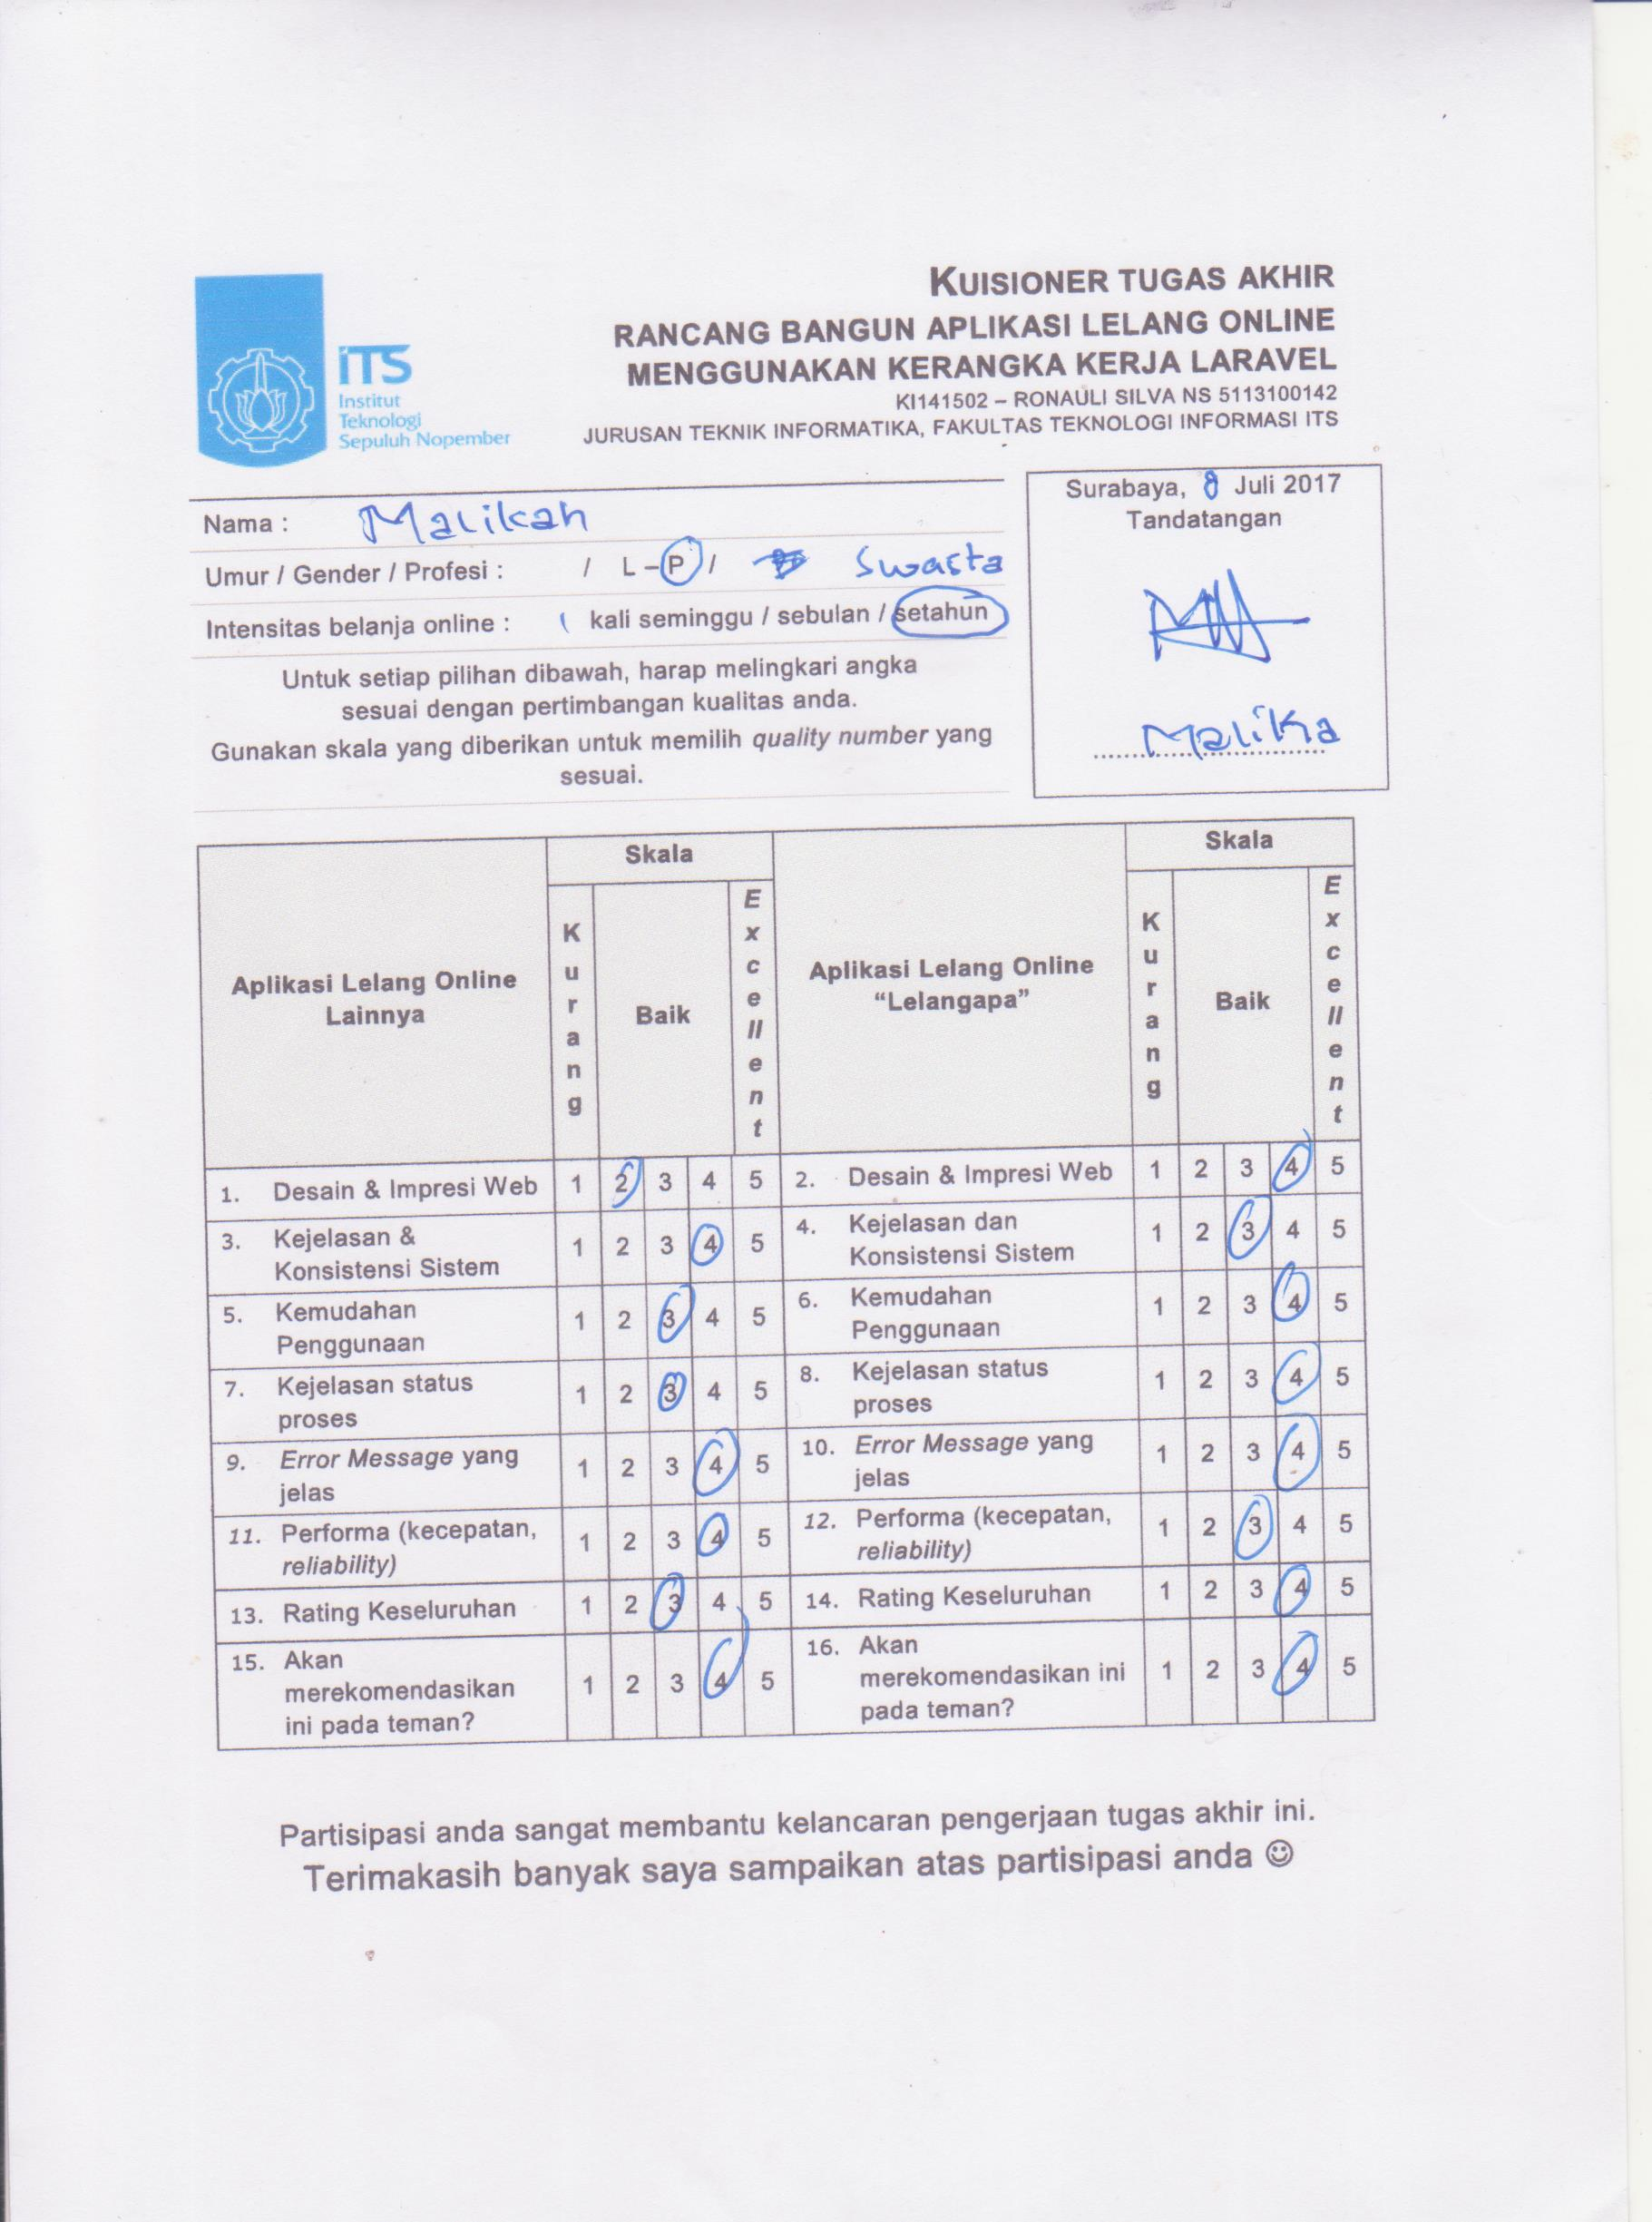
\includegraphics[width=\textwidth]{images/bab5/ujipengguna/4.jpg}
	\caption{Kuisioner Pengguna 4}
	\label{quest-4}
\end{figure}
\begin{figure}[]
	\centering
	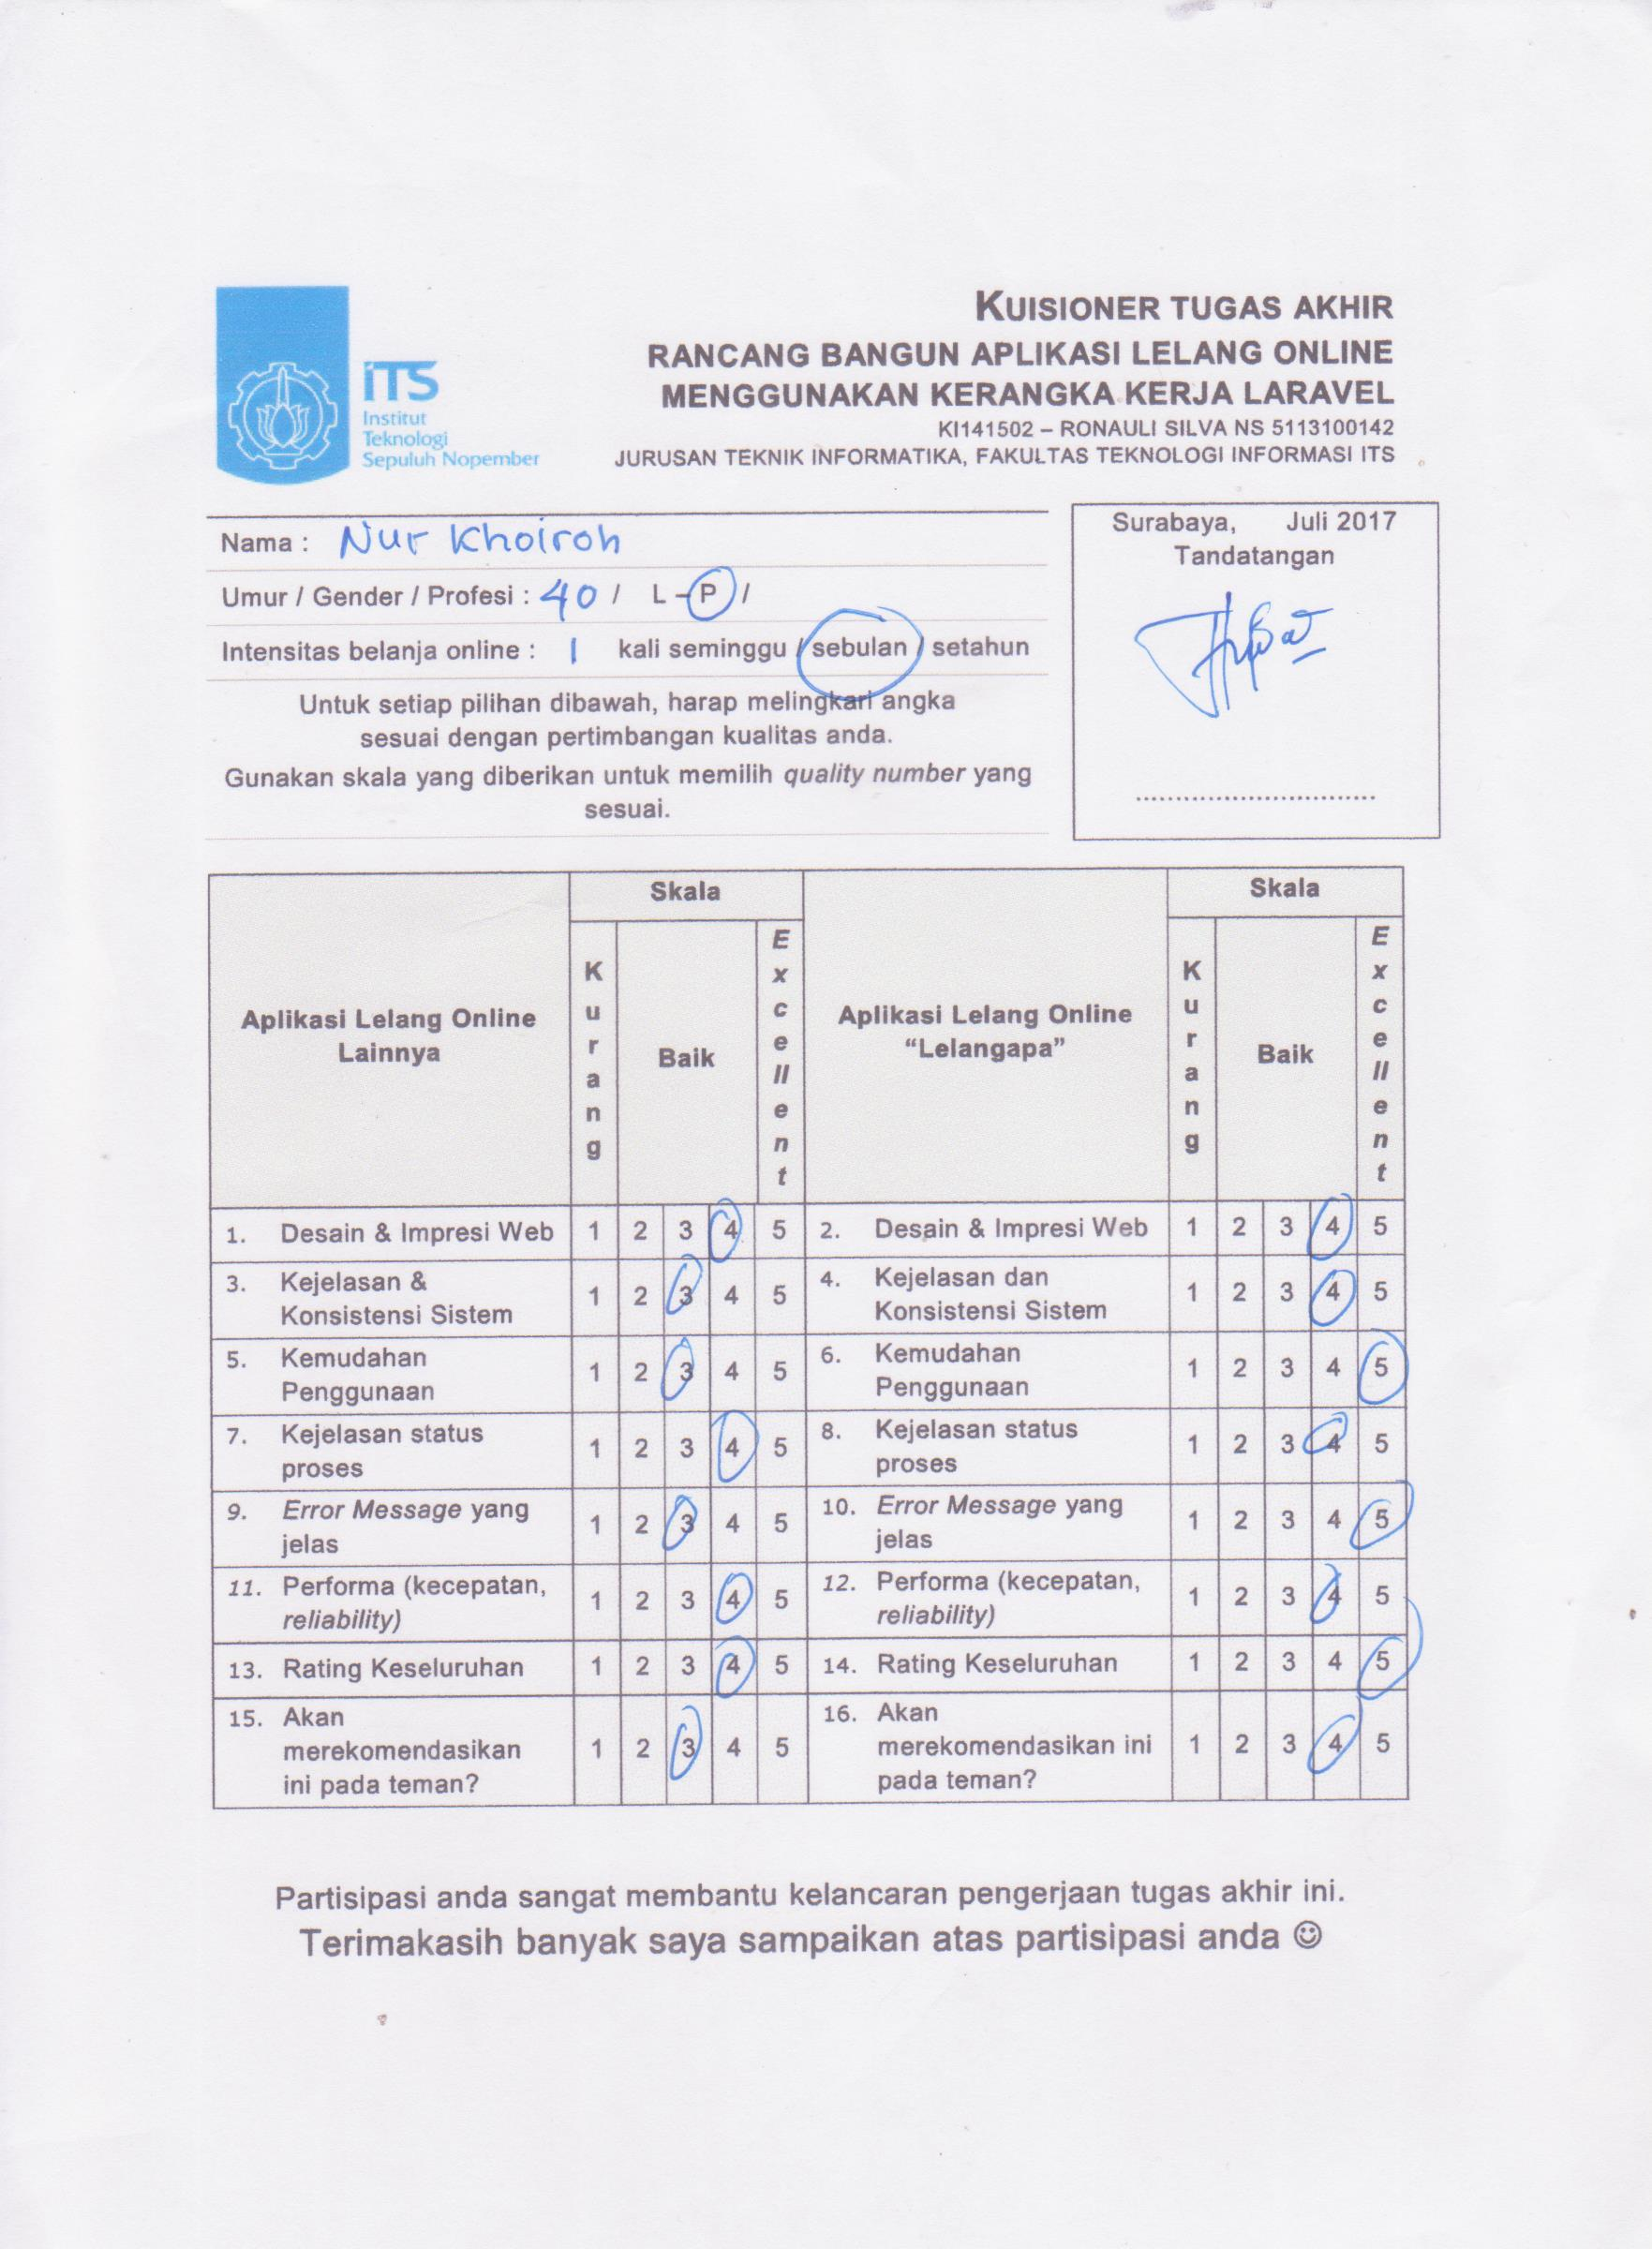
\includegraphics[width=\textwidth]{images/bab5/ujipengguna/5.jpg}
	\caption{Kuisioner Pengguna 5}
	\label{quest-5}
\end{figure}
\begin{figure}[]
	\centering
	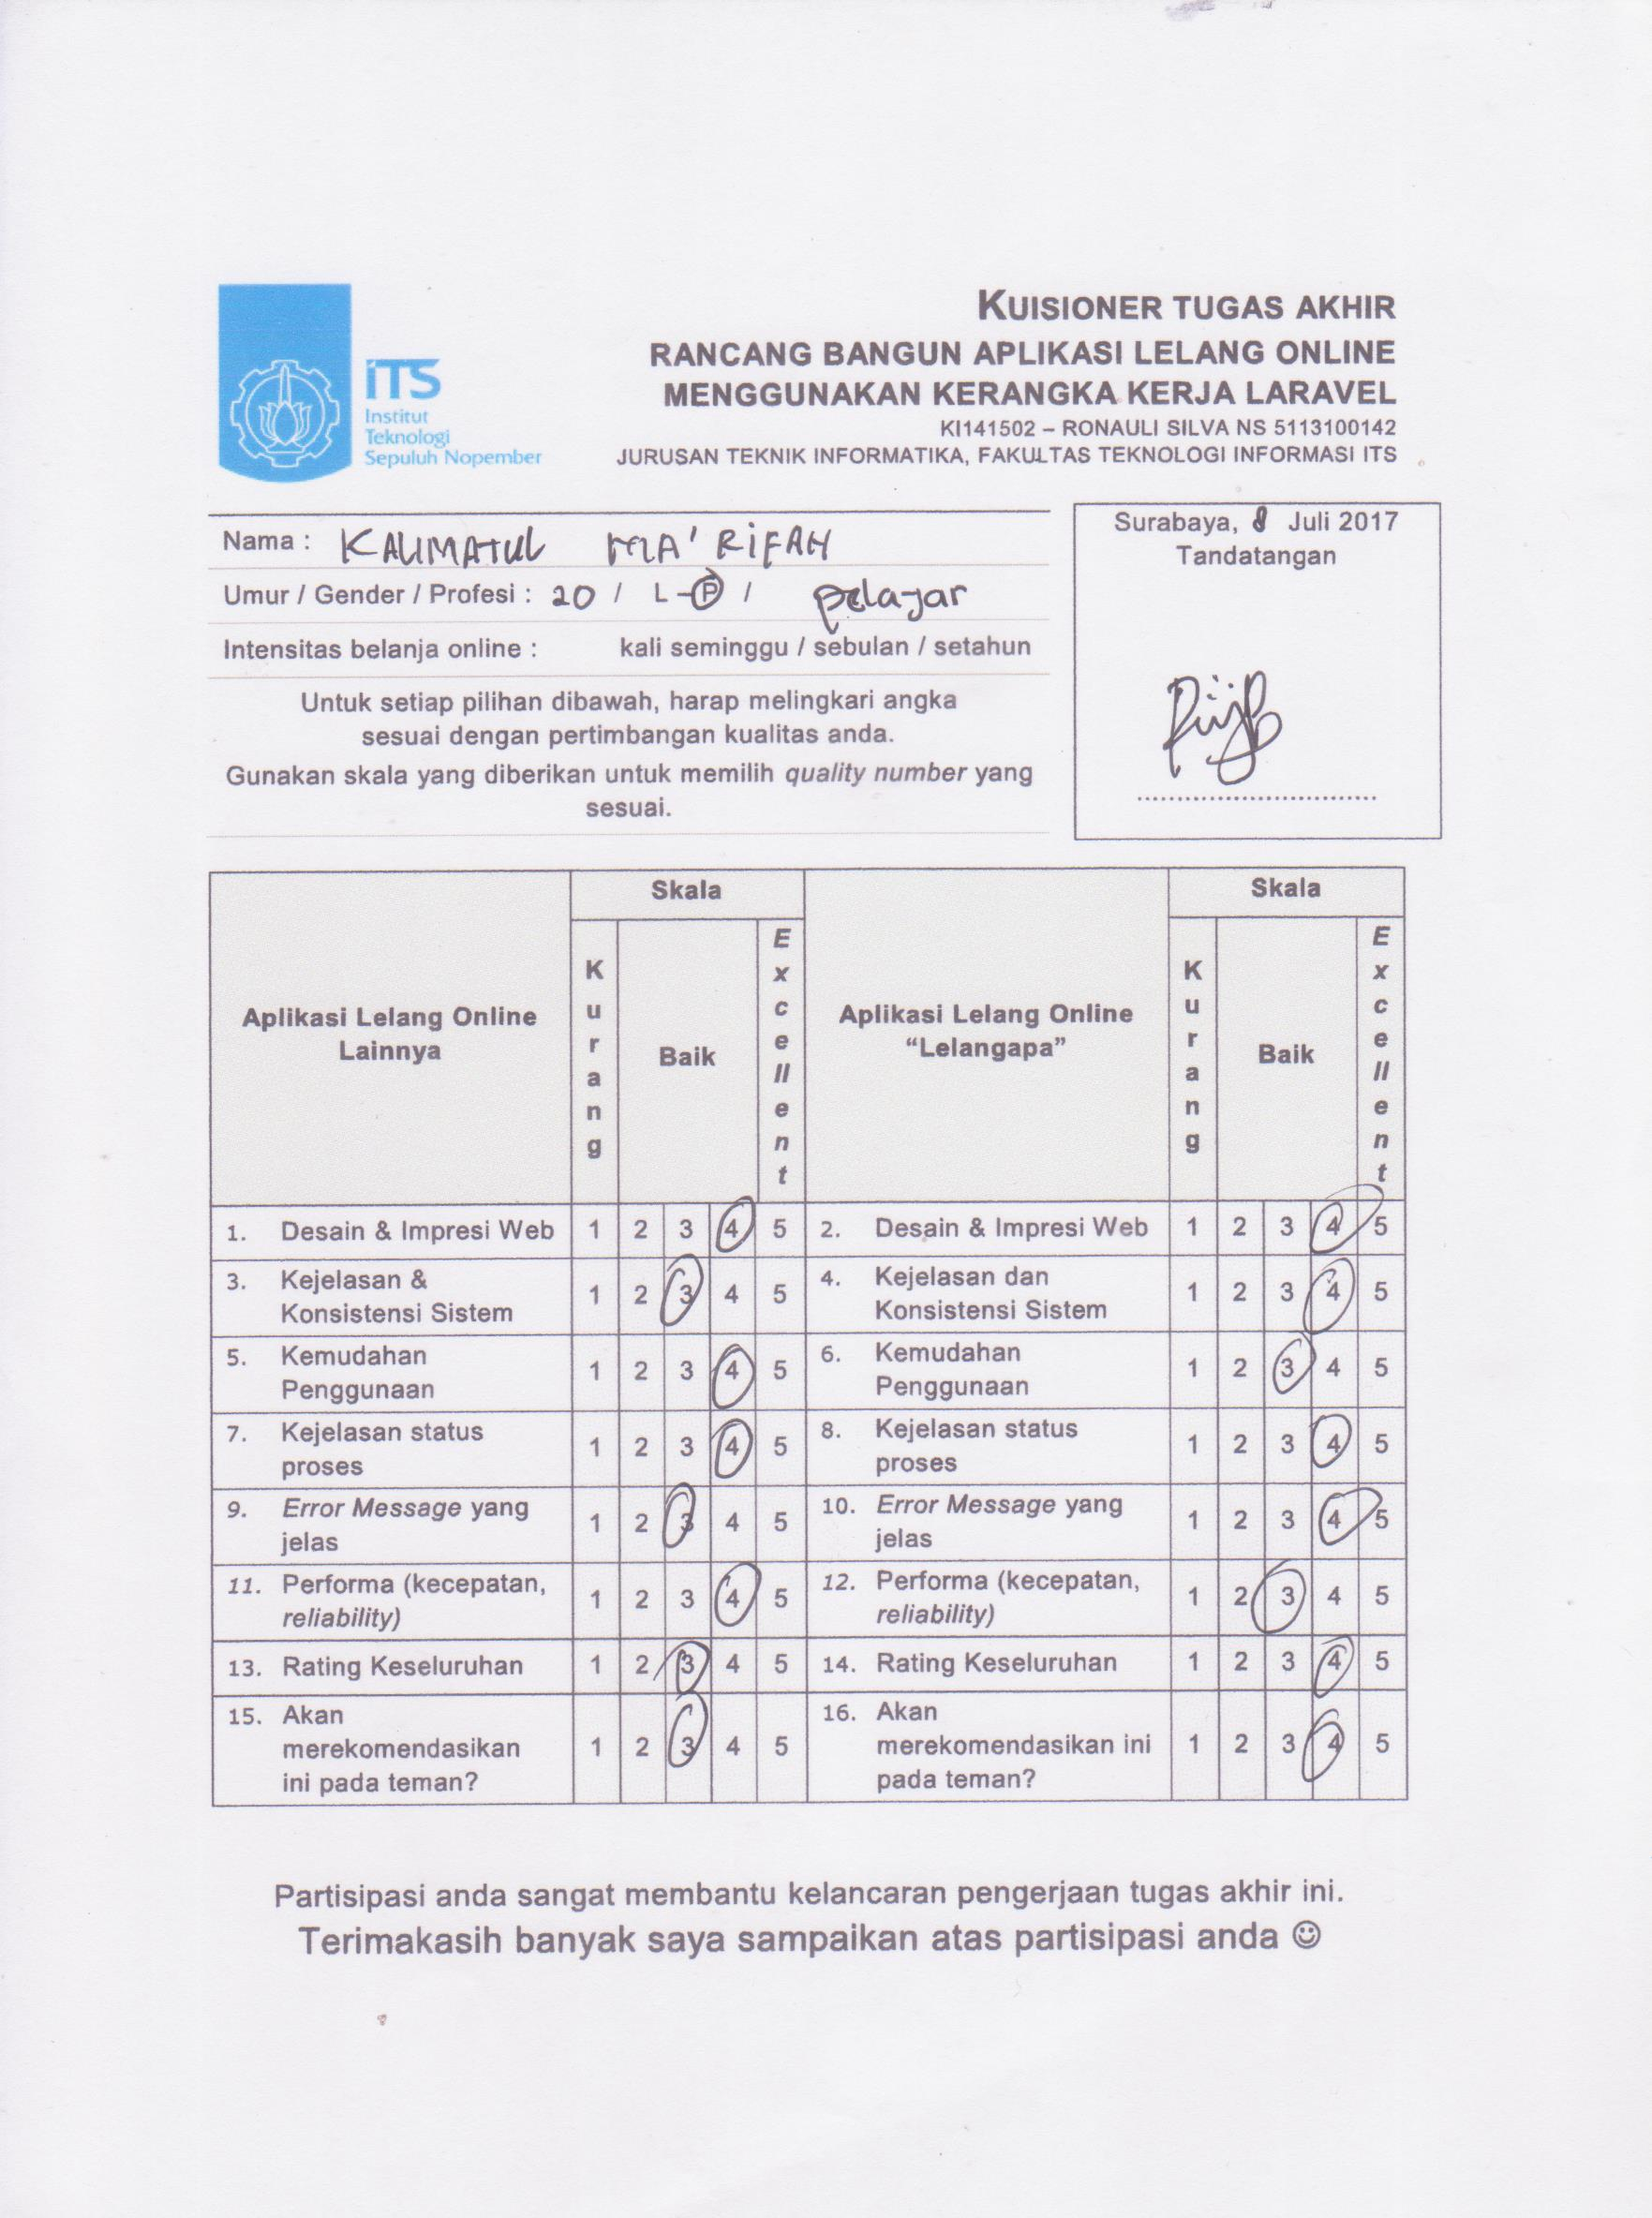
\includegraphics[width=\textwidth]{images/bab5/ujipengguna/6.jpg}
	\caption{Kuisioner Pengguna 6}
	\label{quest-6}
\end{figure}
\begin{figure}[]
	\centering
	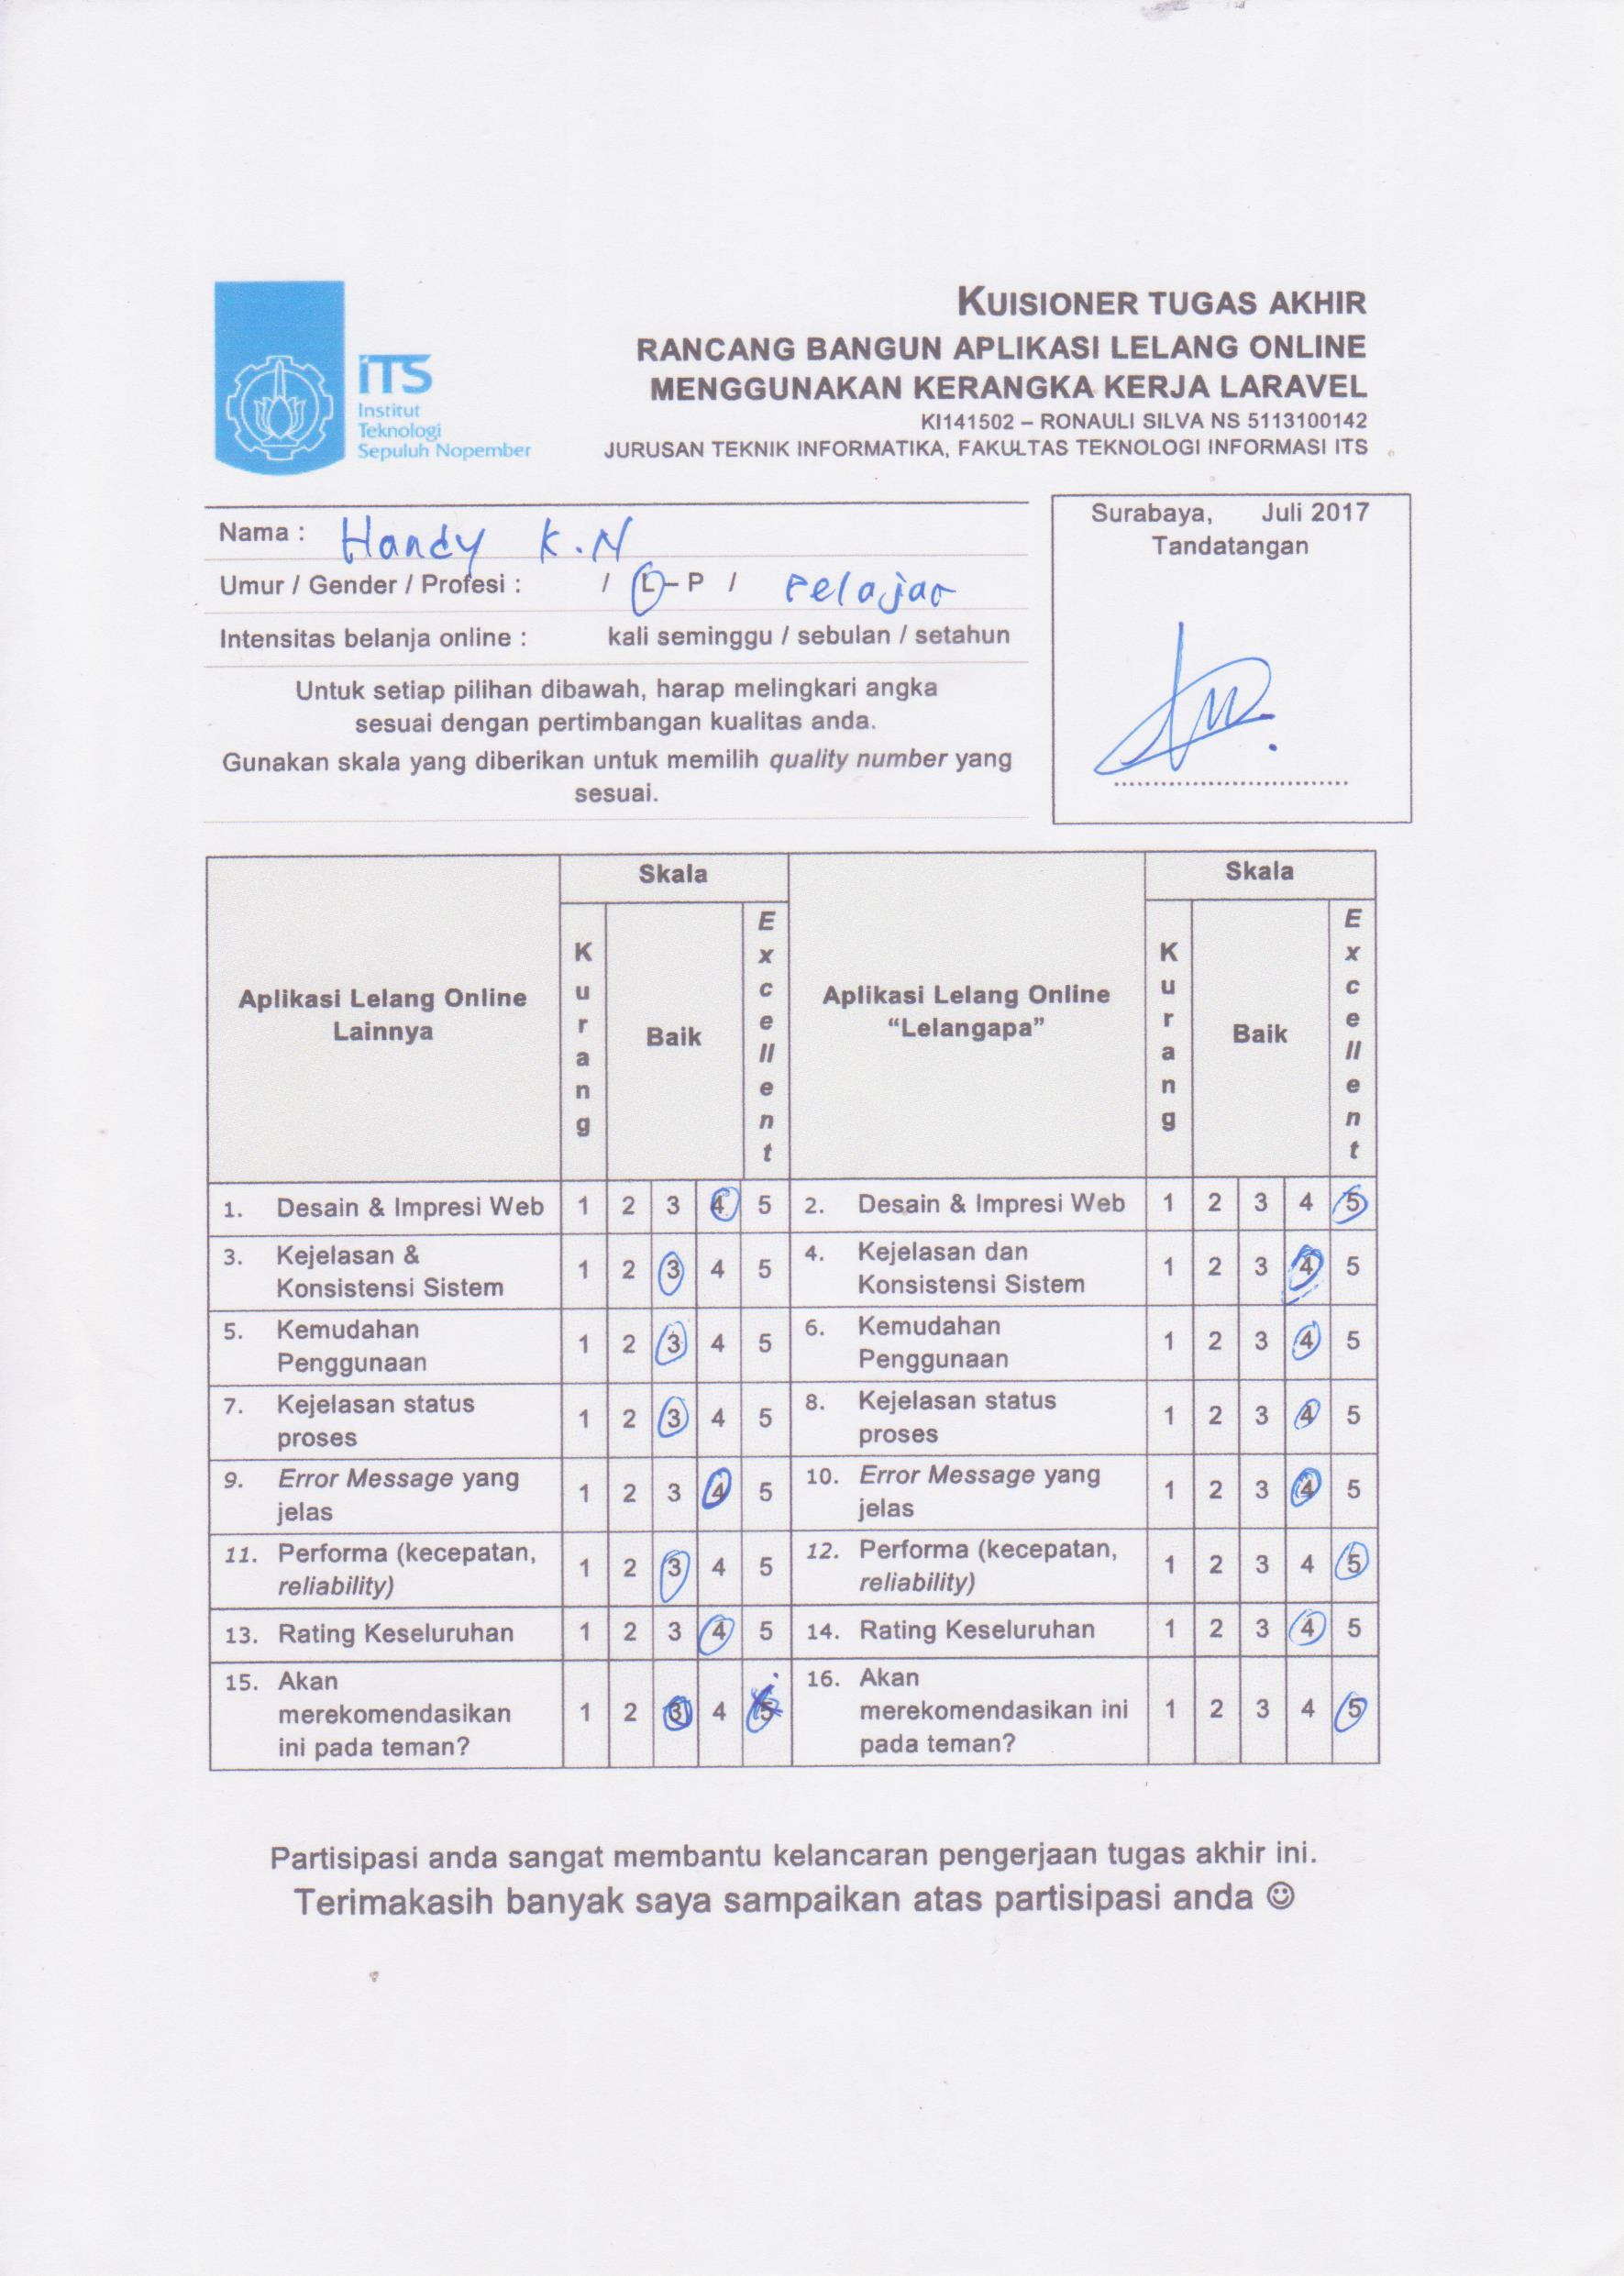
\includegraphics[width=\textwidth]{images/bab5/ujipengguna/7.jpg}
	\caption{Kuisioner Pengguna 1}
	\label{quest-7}
\end{figure}
\begin{figure}[]
	\centering
	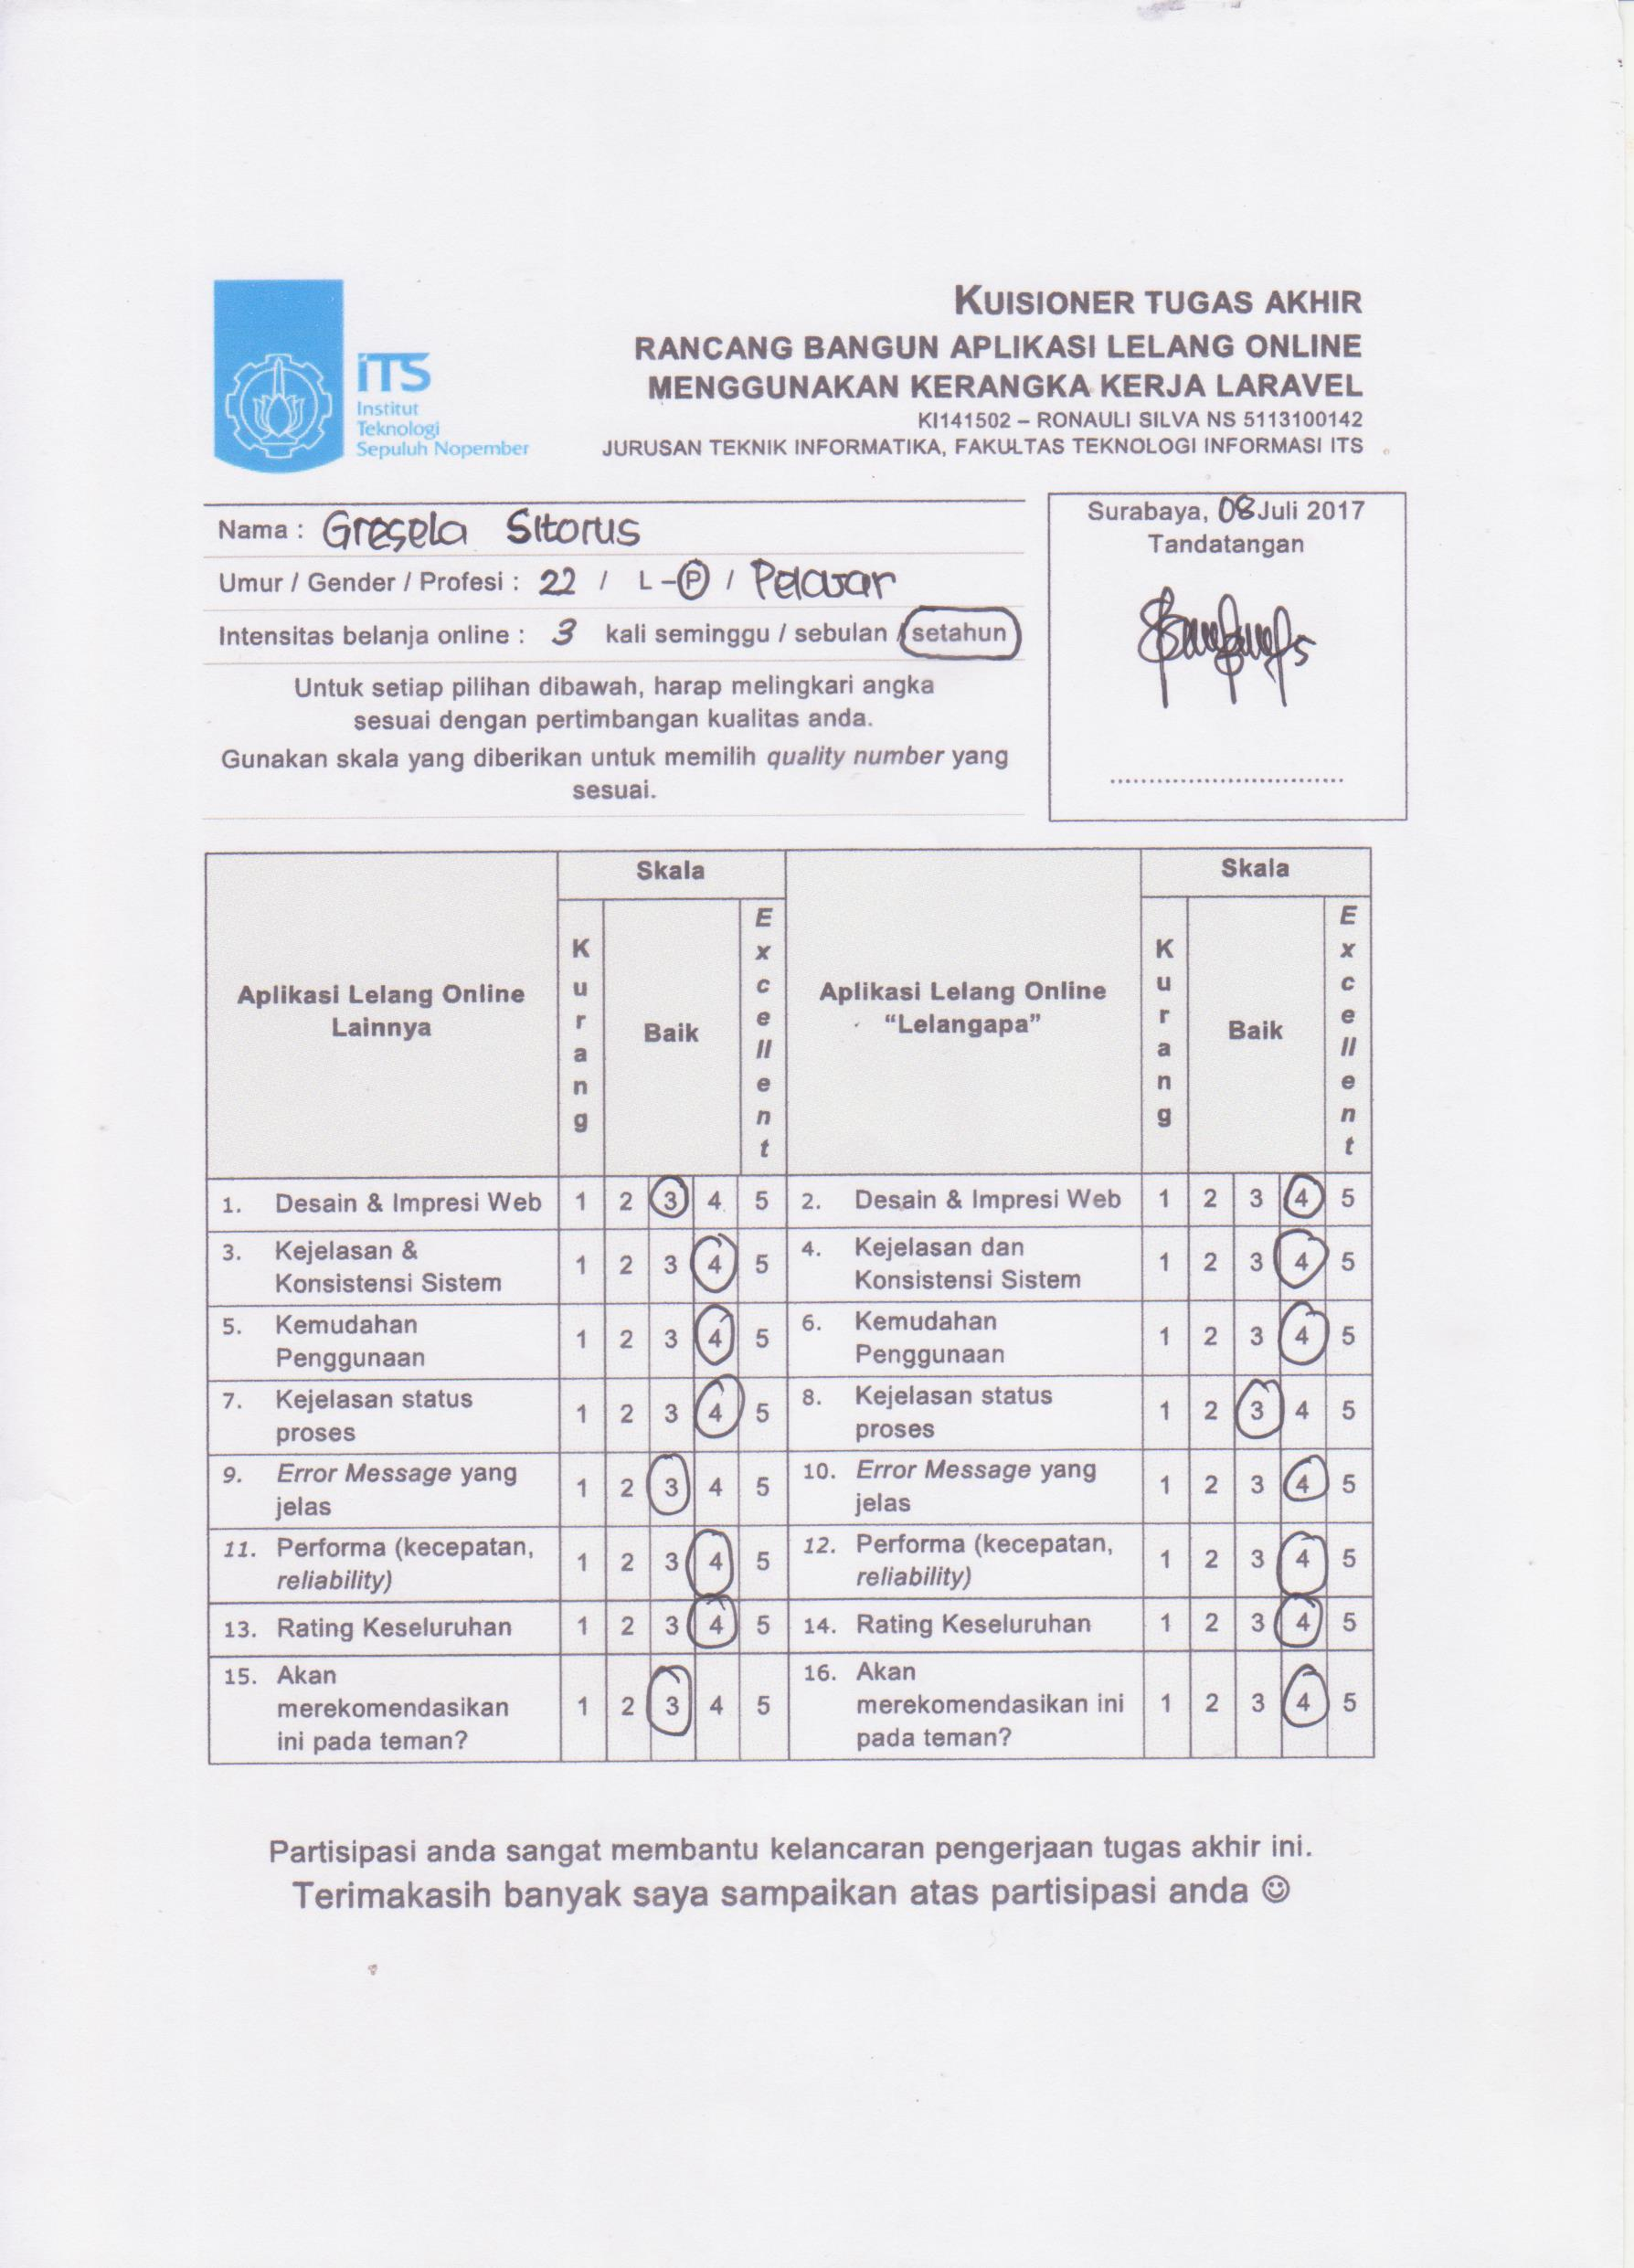
\includegraphics[width=\textwidth]{images/bab5/ujipengguna/8.jpg}
	\caption{Kuisioner Pengguna 8}
	\label{quest-8}
\end{figure}
\begin{figure}[]
	\centering
	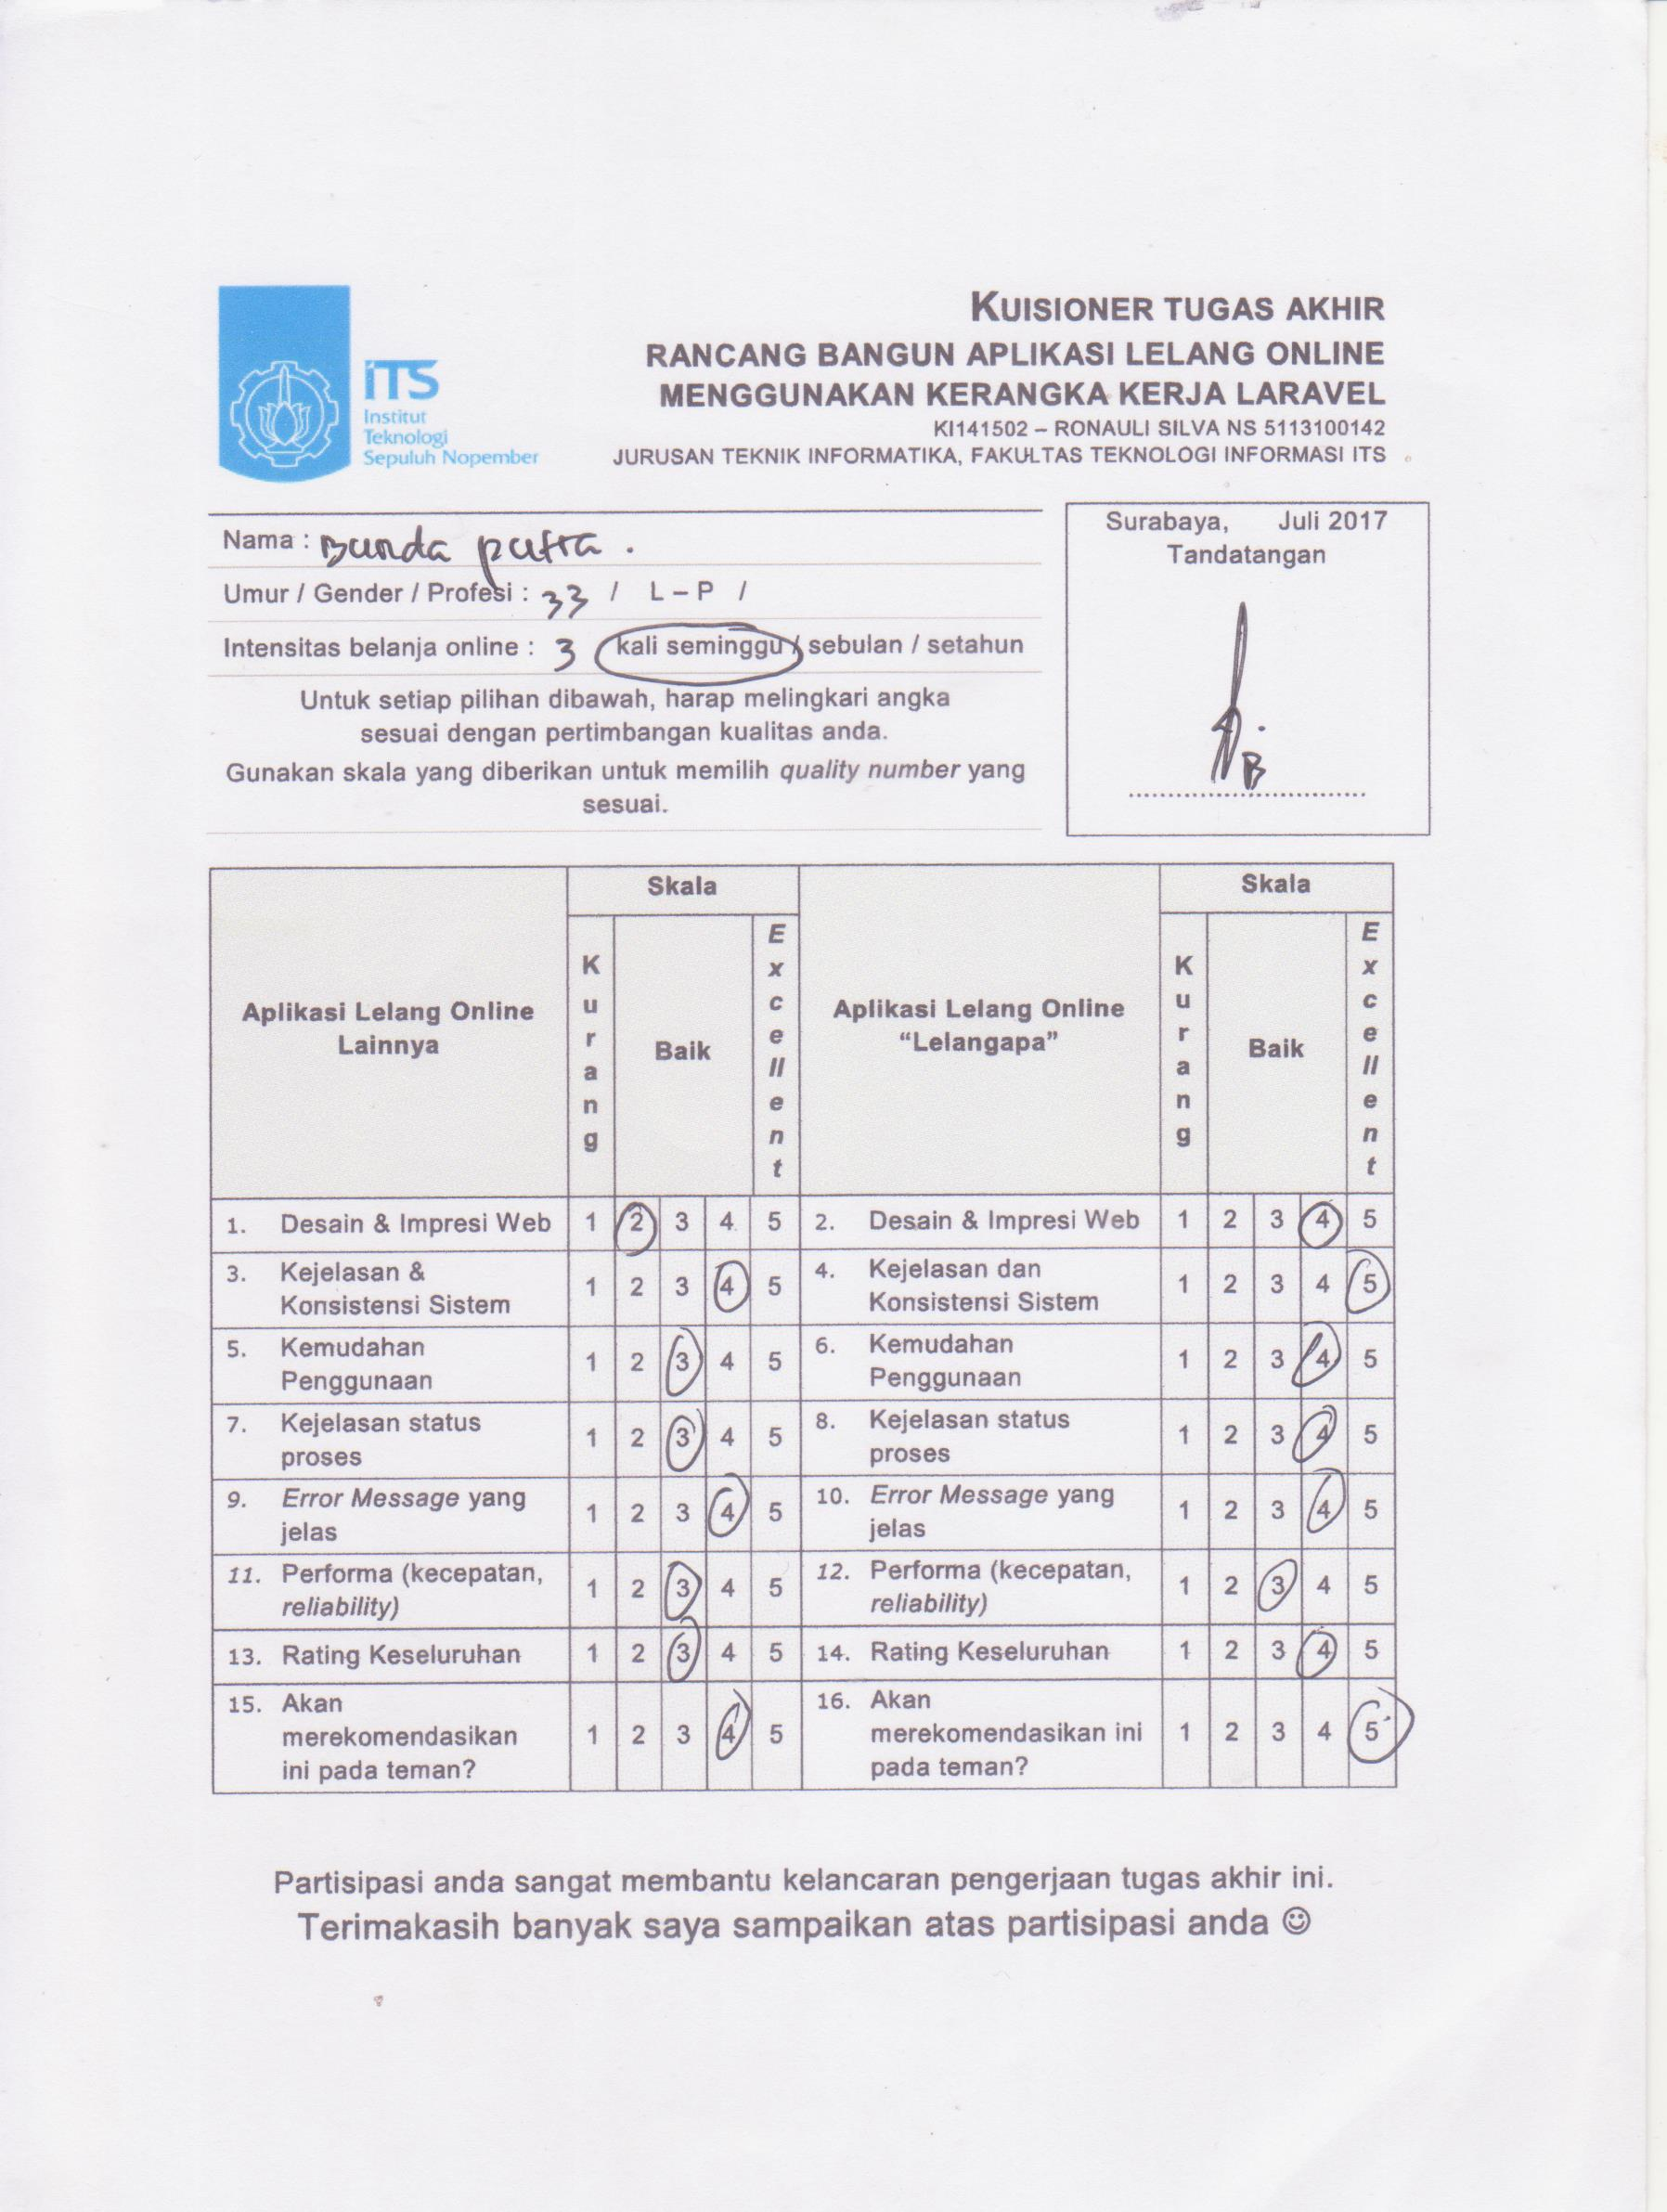
\includegraphics[width=\textwidth]{images/bab5/ujipengguna/9.jpg}
	\caption{Kuisioner Pengguna 9}
	\label{quest-9}
\end{figure}
\begin{figure}[]
	\centering
	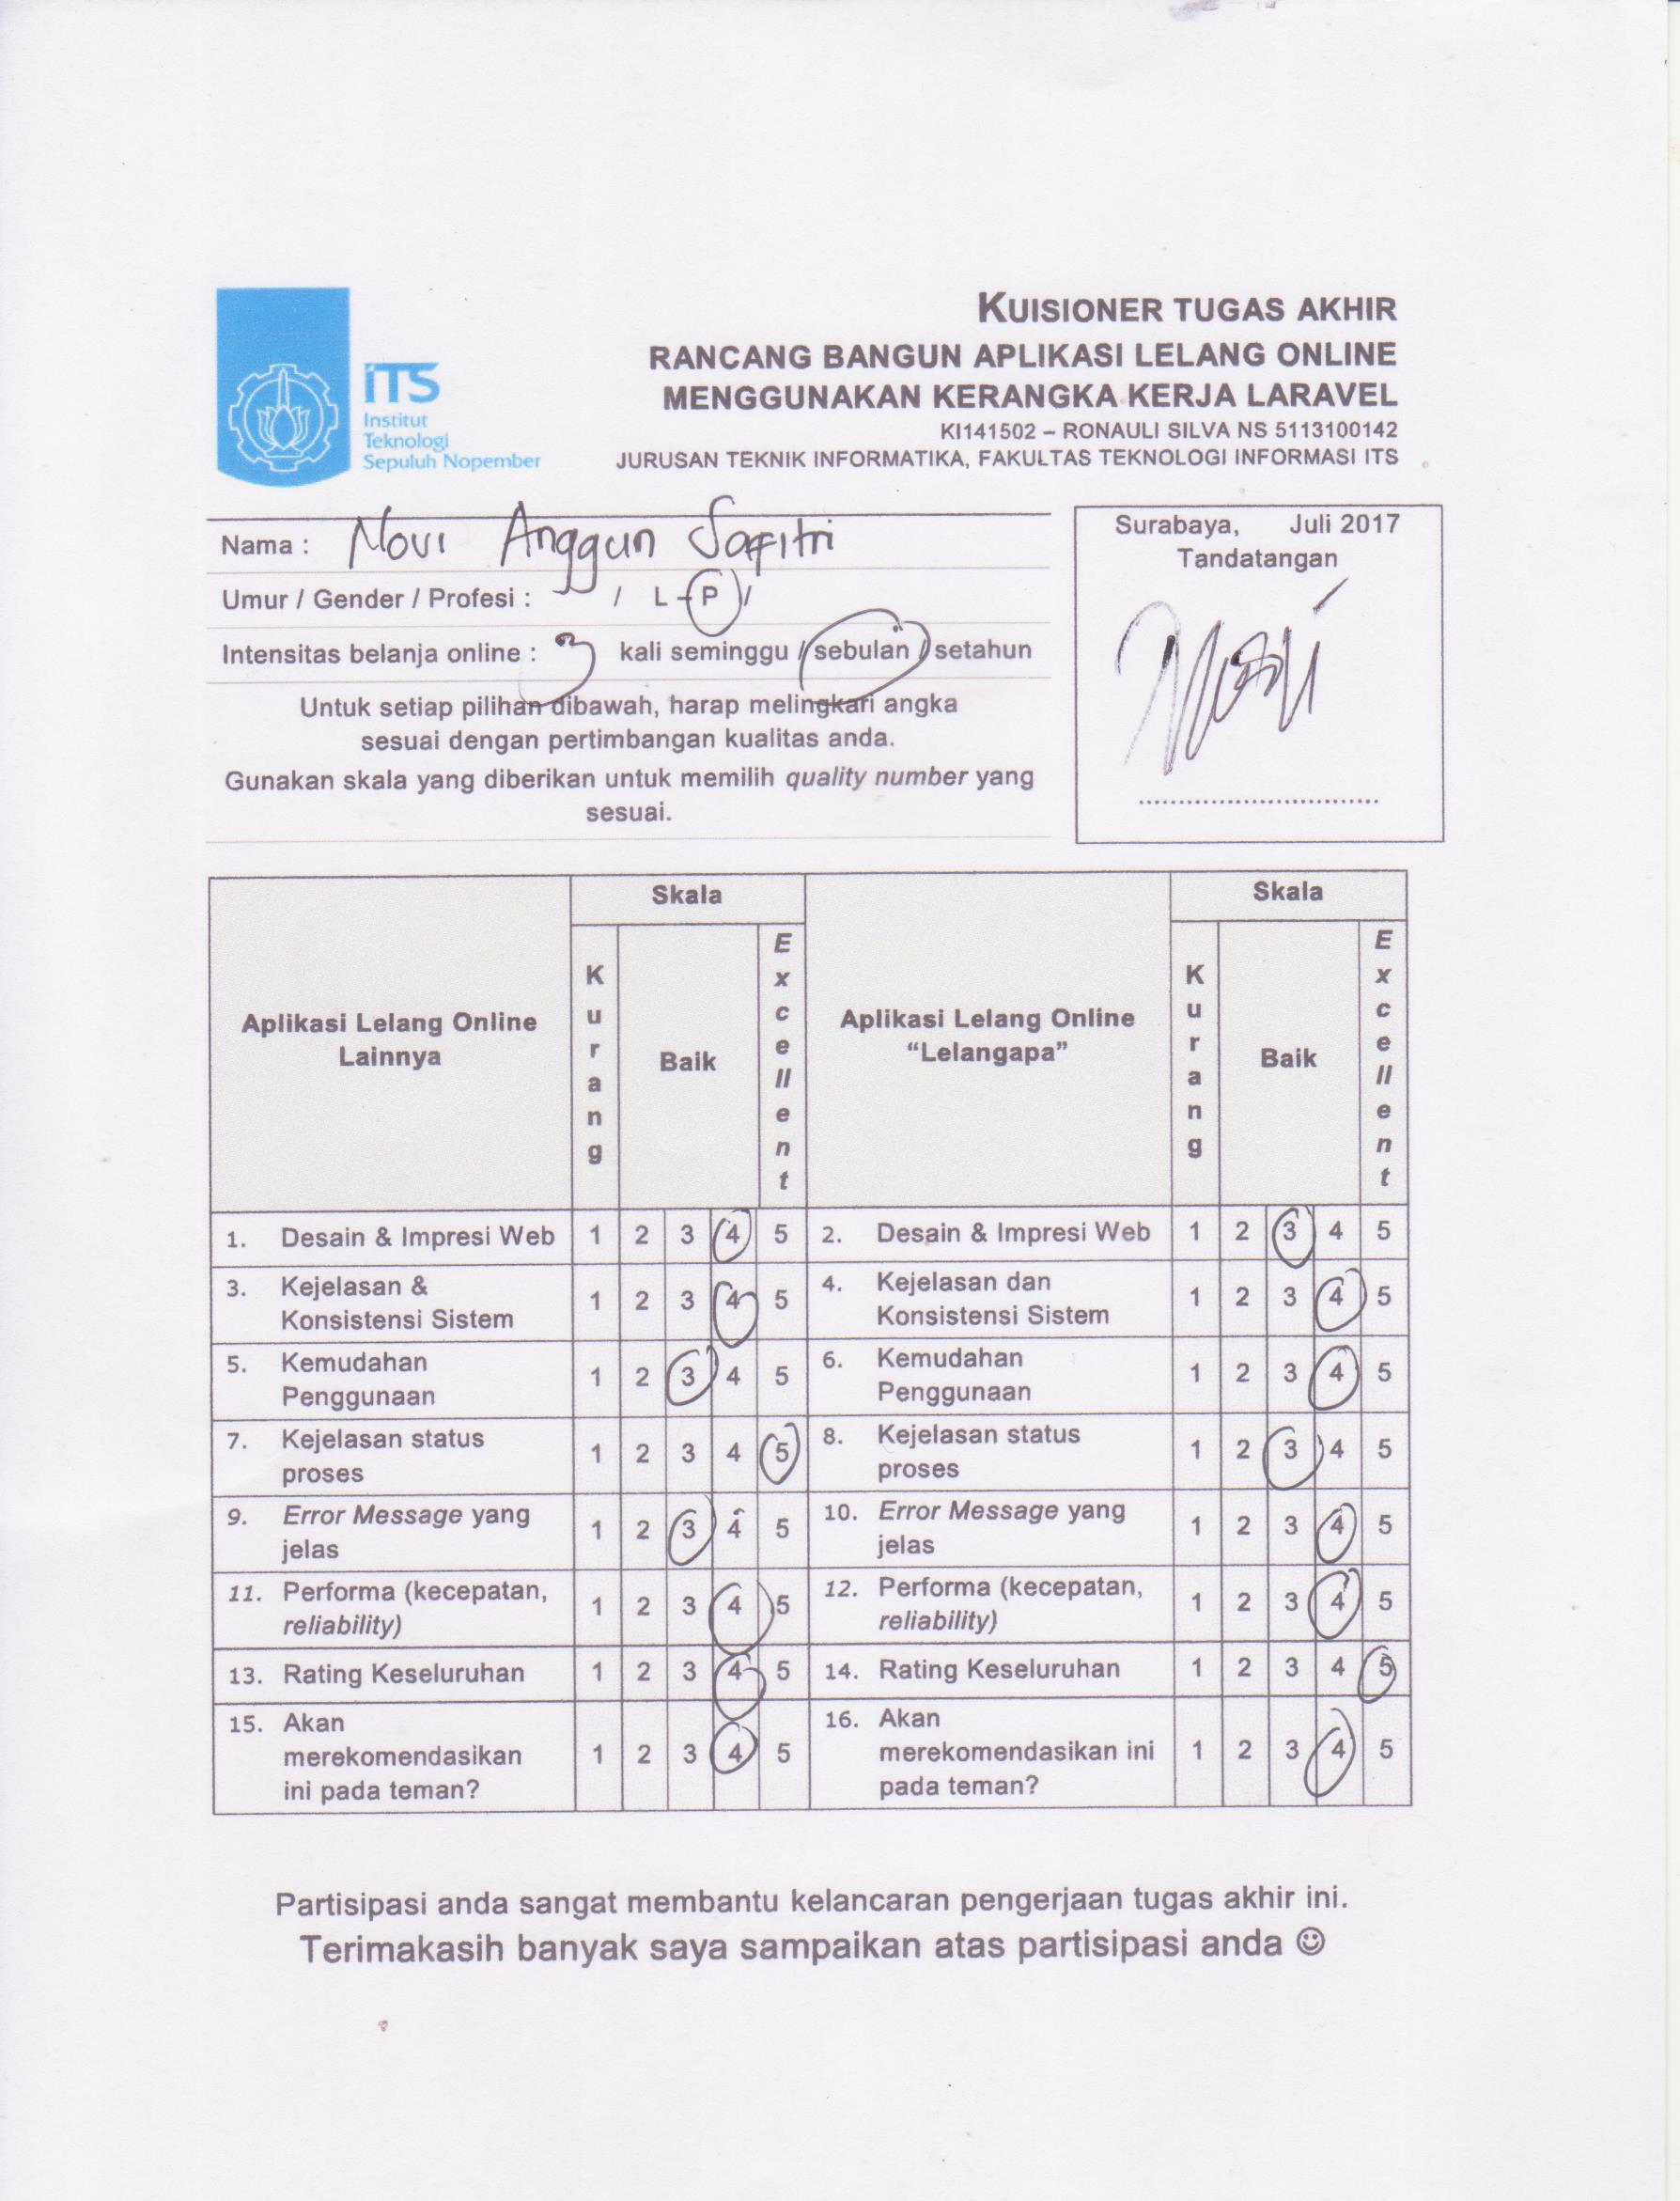
\includegraphics[width=\textwidth]{images/bab5/ujipengguna/10.jpg}
	\caption{Kuisioner Pengguna 10}
	\label{quest-10}
\end{figure}
\begin{figure}[]
	\centering
	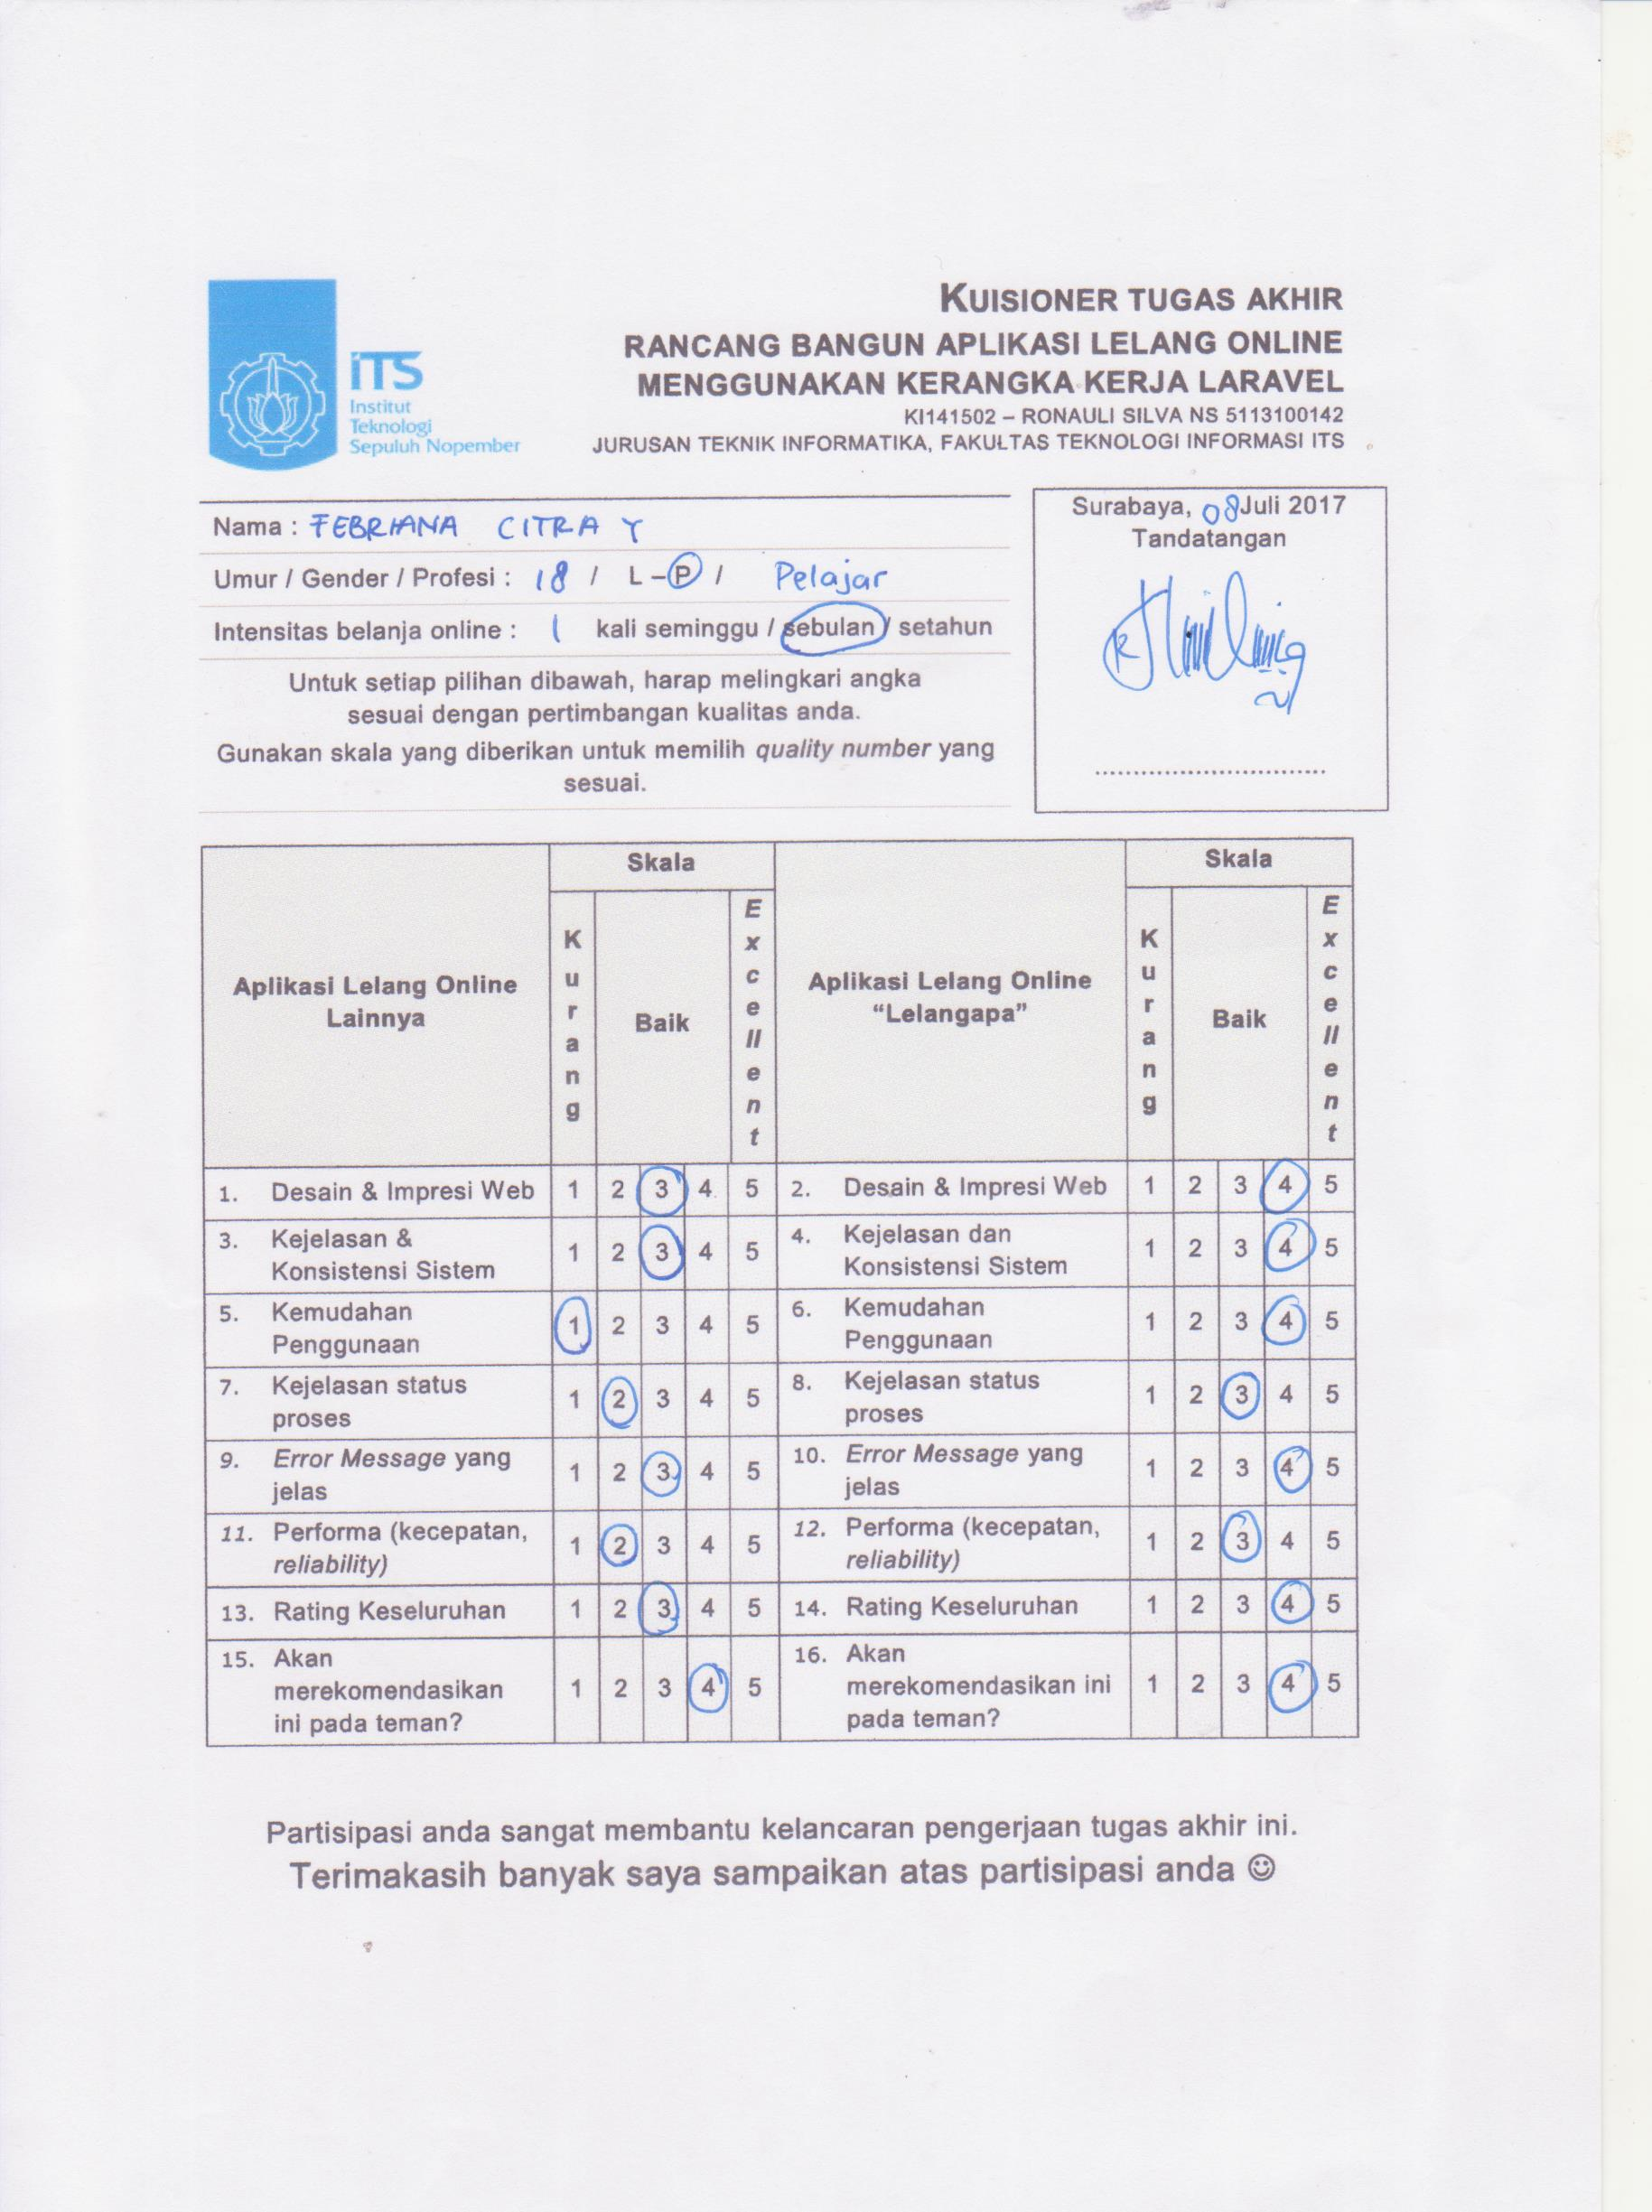
\includegraphics[width=\textwidth]{images/bab5/ujipengguna/11.jpg}
	\caption{Kuisioner Pengguna 11}
	\label{quest-11}
\end{figure}

